\documentclass[11pt]{report}

% to make < and > work
\usepackage[T1]{fontenc}
% for appendices
%\usepackage[toc,page]{appendix}
% CPS equations
\usepackage{amsmath}
\usepackage{stmaryrd}
% Average symbol
\usepackage{amssymb}
% Grammar
\usepackage{syntax}
% Operational semantics
\usepackage{semantic}
% Source code listings
\usepackage{listings}
\lstset{frame=single, numbers=left, basicstyle=\ttfamily}
% Diagrams
\usepackage{graphicx}
% Graph
\usepackage{tikz}
\usepackage{pgfplots}
% Chapter number and name on one line
\usepackage{titlesec}
\titleformat{\chapter}[hang] 
{\normalfont\huge\bfseries}{\thechapter}{1em}{} 

% No new page after chapter
\makeatletter
\renewcommand\chapter{\par%
  \thispagestyle{plain}%
  \global\@topnum\z@
  \@afterindentfalse
  \secdef\@chapter\@schapter}
\makeatother



%%%%%%%%%%%%%%%%%%%%%%%%%%%%%%%%%%%%%%%%%%%%%%%%%%%%%%%%%%%%%%%%%%%%%%%%%%%%%%%%%

\title{LJSP - A LISP to asm.js compiler}
\author{Jan S\"ondermann}
\date{\today}

% Commands to make CPS equations easier to write
\newcommand{\eqdef}{\stackrel{\text{def}}{=}}%
\newcommand{\cpstrans}[1]{\ensuremath{\mathcal{K}\llbracket #1 \rrbracket}}

%%%%%%%%%%%%%%%%%%%%%%%%%%%%%%%%%%%%%%%%%%%%%%%%%%%%%%%%%%%%%%%%%%%%%%%%%%%%%%%%%

\begin{document}

% TODO LIB consistent names for stages


% TODO END nicer title page
\maketitle

% TODO END word count on this page
\begin{center}
\textbf{Originality avowal}
\end{center}

I verify that I am the sole author of this report, except where explicitly stated to the contrary.

I grant the right to King's College London to make paper and electronic copies of the submitted work for purposes of marking, plagiarism detection and archival, and to upload a copy of the work to Turnitin or another trusted plagiarism detection service.\\

\begin{flushright}
Jan Söndermann \\
\today
\end{flushright}
\newpage
			
\begin{center}
\textbf{Abstract}
\end{center}
Over the course of the last decade, JavaScript has turned from an insignificant scripting language to one of the most widespread and commonly used programming languages in existence. The ubiquity of web browsers paired with the exclusivity of JavaScript in web programming have caused the language to be used in increasingly complex applications. This has made performance a top priority for browser developers.

The speed at which JavaScript code can be executed has improved greatly over the last few years, but can still be limiting when building larger web applications. One of the most hotly discussed topics in the community of JavaScript developers in 2013 was the release of asm.js, a small, statically typed subset of JavaScript that can be compiled to efficient machine code. Asm.js promises huge speed gains over plain JavaScript when used as the compilation target for other languages.

To evaluate this new technology and see if asm.js can live up to the hype surrounding it, we design a language called LJSP and build a compiler that compiles LJSP to asm.js. We further implement a ray tracer that serves as a benchmark for different reimplementations of small parts of the ray tracer in asm.js.

\newpage

\begin{center}
\textbf{Acknowledgements}
\end{center}
I would like to thank my supervisor Dr. Christian Urban for supervising my project and for providing me with both guidance and freedom over the course of the year.
% TODO LIB more
\newpage

\tableofcontents
\listoffigures

\newpage

\chapter{Introduction}
One of the main trends of today's Internet is the shift from traditionally offline or standalone programs to online applications on the web. This phenomenon, often called "Web 2.0", is exemplified in the success of web applications such as GMail and Facebook. 

This success of the web has brought with it the rise of the programming language it is build on: JavaScript, the only language supported by all major browsers. Statistics, such as the number of repositories created on GitHub (a popular code sharing website) using JavaScript, reflect this success. In 2013, JavaScript led this list by a substantial margin \cite{githubarchive, topgithub}\footnote{Running the query given at \cite{topgithub} adjusted to include the entire year of 2013 yields $498467$ repositories for JavaScript and $395097$ for Ruby on the second place.}.

Since JavaScript is no longer confined to being used for simple animations and input-validation tasks, the complexity of web apps has increased tremendously. Modern JavaScript frameworks, such as Ember.js or Meteor use the full register of functionality the language offers. These JavaScript frameworks are just as complex as traditional web frameworks that use other languages such as Ruby or Python.

Unfortunately, this proliferation of JavaScript has taken the language far beyond the tasks it was initially designed for. Additionally, there is a widespread consensus that the language has many shortcomings in its design. Brendan Eich, the creator of JavaScript, writes \cite{brendeich} about its early history:
\begin{quote}
In April 1995 I joined Netscape in order to "add Scheme to the browser." [...]

So in 10 days in May 1995, I prototyped "Mocha," the code name Marc Andreessen had chosen. [...]

To overcome all doubts, I needed a demo in 10 days. I worked day and night, and consequently made a few language-design mistakes (some recapitulating bad design paths in the evolution of LISP), but I met the deadline and did the demo.
\end{quote}

and further in \cite{comparticle}:

\begin{quote}
If I had done classes in JavaScript back in May 1995, I would have been told that it was too much like Java or that JavaScript was competing with Java … I was under marketing orders to make it look like Java but not make it too big for its britches … [it] needed to be a silly little brother language.
\end{quote}


Criticism of JavaScript has mostly focussed on two areas:
\begin{itemize}
% TODO END fix line break
\item Inconsistencies and mistakes in the design of the language. Common examples given for this include the confusion around JavaScript's large number of falsy values (\texttt{0},  \texttt{''}, \texttt{NaN}, \texttt{false}, \texttt{null} and \texttt{undefined}) and its set of reserved keywords, which includes a large number of words not in use by the language but doesn't include \texttt{NaN} and \texttt{undefined}. This makes it necessary to test for \texttt{undefined}ness using \mbox{\texttt{typeof x === 'undefined'}} avoid comparing against a redefined \texttt{undefined}. Further problems include unusual scoping and confusing automatic casts. For a long list of problems with JavaScript, see \cite{jsgoodparts}.
\item Slow execution speed. Writing fast interpreters for JavaScript has been an extraordinarily difficult task for browser developers. This is due to the weak typing and generally extremely dynamic nature of JavaScript.
\end{itemize}

Programmers have responded to the first problem in ways that include limiting themselves to a subset of JavaScript that excludes the inconsistent and badly-designed parts (cf. the very popular book "JavaScript: The Good Parts" \cite{jsgoodparts}). Another response has been to create new languages that compile to JavaScript, such as the languages described in the 'Similar Languages' section of the Background Chapter.

The second problem has been partly remedied by a new generation of JavaScript engines spearheaded by Google's V8, released in 2008 as part of Google Chrome. The other browser makers, including Mozilla soon followed by rewriting their own JavaScript engines. These new engines often brought impressive speed gains.

In early 2013, Mozilla released asm.js, a project that claims to take these two approaches to their logical conclusion. It defines an extremely limited, statically typed subset of JavaScript that can be executed very quickly. This subset is intended as compilation targets for high level languages.

The goal of our project is twofold
\begin{itemize}
\item To design such a high level and provide a compiler for it that compiles the language to asm.js.
\item To test the performance of this new language that we called LJSP and compare it to plain JavaScript.
\end{itemize}

To achieve the second goal, the project includes a ray tracer in JavaScript, parts of which were rewritten in LJSP and compiled to asm.js. Rendering time of a 3D scene functioned as a benchmark that made it possible to evaluate the results of the project.

Over the course of the project, a LJSP to asm.js compiler was implemented. This compiler was later extended to also compile LJSP to C and LLVM IR, which in turn were compiled to asm.js code using Emscripten, a program descibed in the next chapter. The different versions of asm.js code were then compared using the included ray tracer.


\chapter{Background}
This chapter will describe the background and context of the LJSP project. It will give technical details of the technologies involved and justify the motivation for starting this project. It will also describe similar and related work done by others.

\section{Relevant technologies}
This section will give an overview of the programs and platforms used in the LJSP project.

\subsection{asm.js}
Asm.js is a small subset of JavaScript that can be compiled to very fast machine code. Benchmarks \cite{asmjsbenchmark} show running times around twice the speed of native code. To showcase the speed of asm.js, researches at Mozilla compiled the Unreal gaming engine to asm.js, producing smooth and stutter free rendering inside the browser \cite{unreal}.

After its release, asm.js has generated enormous interest in the community in places such as \cite{hnthread}. The goal of LJSP is to evaluate the performance achievable with a language that compiles to asm.js and find out if the hype surrounding it is justified. This section will describe the concepts behind asm.js and give a technical description of its specification. The Implementation chapter below will build on this description to explain the asm.js code that the LJSP compiler outputs.

Asm.js is designed as a very limited subset of JavaScript that includes information typically not included in JavaScript code. If the author of asm.js compatible code adds a statement that marks the code as compatible, and the browser of the user viewing a website that includes this code supports asm.js, the JavaScript engine of the browser can use that additional information to compile the code to very efficient machine code. This compilation happens ahead of running the program (this is sometimes called Ahead-of-time-compilation).

The way to opt-in to this optimisation is to add a \texttt{"use asm";} statement to the top of the function that contains the code\footnote{The syntax for this opt-in is copied from the popular and widespread \texttt{"use strict";} directive that makes JavaScript engines less lenient when parsing JavaScript code.}. Supporting browsers (currently only Firefox) will then compile the code and output a string such as "\texttt{successfully compiled asm.js code (total compilation time 25ms)}" in the case of successful compilation to the console when loading this function.

Most of the additional information that asm.js forces the programmer to include in his programs that would typically not be part of idiomatic JavaScript is type information. Unlike JavaScript, asm.js is statically typed, meaning every variable has a type inferable at compile time. The following examples will illustrate this difference. We start with a small function in standard JavaScript shown in Fig. \ref{jssimplefunc}.

\begin{figure}[ht]
\begin{lstlisting}
function add(a, b) {
    return a + b;
}
\end{lstlisting}
\caption{A simple addition function in JavaScript}
\label{jssimplefunc}
\end{figure}

The name of this function suggests that it was probably conceived to add two numbers. It could, however, be called with \texttt{add("hello ", "world");} and would yield the concatenated string \texttt{"hello world"}. Neither is it restricted in the type of numbers it accepts: it can be called with an arbitrary combination of integers and floating point numbers.

The same function restricted to integers in asm.js would look as shown in Fig. \ref{asmjsadder}.

\begin{figure}[ht]
\begin{lstlisting}
function add_ints(a, b) {
    a = a|0;
    b = b|0;
    
    return (a + b)|0;
}
\end{lstlisting}
\caption{An asm.js function that computes the sum of two ints}
\label{asmjsadder}
\end{figure}

The additional lines 2 and 3 are the kind of type information mentioned above. They declare both parameters \texttt{a} and \texttt{b} to be of type int. In other languages such as C, the parameters would be written as \texttt{int a, int b}. In valid asm.js, all parameters to every function get a type assigned at the very top of the function. The somewhat strange syntax for this type declaration is explained in detail in the next few paragraphs.

The other change from the original JavaScript version to the asm.js version of the addition function is the inclusion of a bitwise OR\footnote{The pipe symbol \texttt{|} is used for bitwise OR in JavaScript} with 0 to the result of the sum in line 5. This is necessary because of the other main feature of asm.js besides the possibility of compiling it efficiently:

The asm.js specification \cite{asmjsspec} guarantees that valid asm.js code evaluates to the same result regardless of whether or not the browser has asm.js support. If we consider the situation where the browser does have asm.js support and the function \texttt{add_ints} defined in the example above is called with two very large integers, the compiled, native code would add these two large ints and cause an integer overflow. If, however, the browser does not support asm.js and treats the code as normal JavaScript, adding two integers large enough that normally an overflow would occur causes the result to be cast to a floating point number according to the JavaScript specification.

The bitwise OR in the line \texttt{return (a + b)|0;} ensures that even in the case of missing asm.js support, the result returned by the function would still be an overflowed integer. The reason for this is that following the JavaScript specification, the bitwise OR with 0 coerces the result to be of type int. These expressions are therefore known as "type coercions" and asm.js makes heavy use of them.

To illustrate type coercions with an example, consider the interactive JavaScript session shown in Fig. \ref{jstypecoercion}.

\begin{figure}[ht]
\begin{lstlisting}
> 2147483647 + 1
2147483648
> (2147483647 + 1) |0
-2147483648
\end{lstlisting}
\caption{Demonstrating type coercion in the JavaScript console}
\label{jstypecoercion}
\end{figure}

$2147483647$ is equal to $2^{31}-1$, the largest value that can be saved in a 32 bit signed integer variable. If we add one to this value without any coercion, the result is transparently cast to a double and returned. If, however, we include a type coercion, the result overflows to $-2^{31}$.

Asm.js uses type coercions both to ensure that the code produces the same result in all circumstances and as type annotations for parameters as Fig. \ref{asmjsadder} demonstrated.

In the remaining part of this section, will give an overview of the asm.js specification with a restriction on the parts that are relevant to the LJSP compiler. For reasons of space, this overview will leave out information that is unimportant for our project and is not meant as a general introduction to all the specifics of asm.js.

Asm.js code is organised in asm.js modules which are made up of a surrounding function that includes the \texttt{"use asm";} directive mentioned at the beginning of this section. As parameters, it can take a \texttt{stdlib} object that makes it possible to import certain functions from the JavaScript standard library into the asm.js module and an \texttt{ArrayBuffer}\footnote{In JavaScript, \texttt{ArrayBuffer} objects represent blocks of memory.} object often called "heap". Besides this, the function can include:
\begin{itemize}
\item Global variables
\item Functions
\item Function tables
\item A return statement
\end{itemize}

Valid asm.js functions include enough type information to be statically typable as explained above. They can declare variables, perform arithmetic operations on these variables, branch using \texttt{if} statements, read from and write to the heap and call functions either by name or by looking them up in a function table.

Function tables in asm.js are arrays of functions. These arrays must be of a size equal to a power of two. When using a function table to call a function, the variable that is used as index must be masked bitwise to ensure that function table lookup never failes with an out of bounds error \cite{asmjspdf}. This is a complex idea best illustrated with an example. Suppose our code includes a function table \texttt{ftable} that contains $8$ functions, and a variable \texttt{x} that holds the index to a function in \texttt{ftable} that we would like to call. This call could be achieved with the statement \texttt{ftable[x \& 7](param1, param2, ...);}. The bitwise AND with $7$, or $111_2$ in binary, ensures that regardless of the value \texttt{x} holds, no out of bounds error can occur, as the result of the bitwise AND will always be between 0 and 7. The reason asm.js allows multiple function tables is because all functions in a table must have the exact same type signature in parameters and return types.

The return statement at the end can make functions defined inside the module visible to the outside.

Concluding this section, we will explain the \texttt{ArrayBuffer} object mentioned above and the way that asm.js modules interact with it. In JavaScript, \texttt{ArrayBuffer} objects represet blocks of memory that can hold any kind of data. It is, however, not possible to access this memory directly using the \texttt{ArrayBuffer} object. Instead, a subclass of another class, \texttt{ArrayBufferView} is created as a view on the \texttt{ArrayBuffer}. These views all interpret the memory held in the \texttt{ArrayBuffer} to be of a specific type. The example given in Fig. \ref{arraybufferexample}, created with the Chrome JavaScript console, illustrates these classes and their usage.

\begin{figure}[ht]
\begin{lstlisting}
> var buf = new ArrayBuffer(12);  // 12 bytes
> var i16view = new Int16Array(buf);
> var i32view = new Int32Array(buf);

> i16view;
[0, 0, 0, 0, 0, 0]

> i32view;
[0, 0, 0]

> i32view[0] = 42; i32view[1] = 65536;

> i32view;
[42, 65536, 0]
> i16view;
[42, 0, 0, 1, 0, 0]

> new Float32Array(buf)
[5.885453550164232e-44, 9.183549615799121e-41, 0]
\end{lstlisting}
\caption{Demonstration of the \texttt{ArrayBuffer} class and its views}
\label{arraybufferexample}
\end{figure}

In line 1 of Fig. \ref{arraybufferexample}, an \texttt{ArrayBuffer} that holds 12 bytes of memory gets created. In lines 2 and 3, we create two views to this \texttt{ArrayBuffer}. Both are of type integer, but \texttt{i16view} interprets the memory to be made up of ints with 2 bytes (16 bits), whereas \texttt{i32view} is a view that interprets the buffer as ints with length 4 (32 bits). This explains the result of the next two statements in lines 5 and 8: i16view is an array of length 6, because the 12 bytes of the \texttt{ArrayBuffer} get grouped into 6 ints of length 2 each. Equivalently i32view: its length is $12/4 = 3$.

In line 11, the four byte view is used to write two numbers to the array. The result of this is confirmed in lines 13 and 14 which reflect that change. Line 15 proves that the views do not hold any data by themselves but are all views to the same underlying \texttt{ArrayBuffer}. Note how the value $65536 = 2^{16}$ overflows from the less significant two bytes at \texttt{i16view[2]} to the next two bytes.

The fact that views interpret the underlying bits to be of a specific type is again exemplified by line 19 which does not, as one might expect, return \texttt{[42.0, 65536.0, 0]}, but instead interprets the bits of the two integers as 32 bit floats. This produces the scrambled values returned by the statement.

Similarly to function table calles explained above, accessing the values in an \texttt{ArrayBuffer} requires addtional safeguards to make sure the result is not undefined. According to the asm.js spec, array dereference expressions must be of the form \texttt{x[(e \& mask) {>}> i]} with \texttt{mask} being equal to the number of bytes in the \texttt{ArrayBuffer}\footnote{Which must be a multiple of $4096$} minus $1$ and \texttt{i} being equal to the number of bytes the data type of the view used for the access is based on (e.g. $4$ in the case of \texttt{Int32View}). In combination, they prevent out-of-bounds accesses by discarding bits larger than the length of the array and shifting the index to the right size for the view. In practise, the mask turned out not to be required in heap access expressions for Firefox to accept the code as valid asm.js.

\subsection{LLVM and Emscripten}
In order to gather more data with which the performance of the compiler could be compared, the project was extended to also interact with LLVM and Emscripten. LLVM is a compiler project that includes and has spawned a large number of tools and programs related to the compilation of programs. At its core, it defines an intermediate representation called LLVM IR and an optimizer for this language. This intermediate representation aims to be a shared interface for front ends that parse programming languages and compile them to LLVM IR and back ends that take LLVM IR code and produce native code for a specific architecture such as x86 or arm. 

While a large number of these front and back ends for various languages and architectures have been written, only one is relevant to the LJSP project: a LLVM IR to JavaScript compiler called Emscripten. Emscripten was written by the same group of researches that invented asm.js; in fact, asm.js was created to fill a need the Emscripten developers had for a better compilation target. They describe the challenges of writing a compiler from LLVM IR, a low-level language, to JavaScript, a high-level language in \cite{emscriptenpapar}.

The LJSP compiler emits both C and LLVM IR code. This generated code can be compiled with Emscripten to asm.js. The Evaluation Chapter will compare the running time of this code that Emscripten emits with the asm.js code that LJSP generates directly.

\subsection{Ray Tracing}
Ever since the first computers were built, programmers have sought ways to generate pictures with programs. Especially with the rise of computer games, this has become a heavily researched area. Ray tracing is one such technique to generate images from description of 3D scenes. Because generating these images is a computationally intensive task, it is suited to be used for benchmarking.

Before we can describe the details of ray tracing, we have to introduce two terms that we will refer to in our explanation: A \textbf{3D Scene} is an arrangement of objects at specific coordinates in 3D space. Object can include shapes such as spheres, cubes or planes, lights and a camera. The \textbf{camera} is not a visible object, but instead gives the perspective an angle from which the scene will be rendered. \textbf{Rendering} denotes the process of generating an image from a 3D scene and the program that does this is called a renderer.

Ray tracing produces relatively impressive results with simple techniques. It works by shooting rays from the camera into the scene. The ray tracer then traces these rays and determines whether they hit an object in the scene. If they do, the process of shooting rays into the scene is repeated recursively with the intersection point as the origin of the rays to achieve photorealistic effects such as reflection. If they don't, black or some other background colour is displayed.

\section{Similar Languages}
Because of the problems with the JavaScript language mentioned in the Introduction, a large number of programming languages that compile to JavaScript or replace it altogether have been developed. These languages all try to fix some of JavaScript's problems.

The most successful of these language is CoffeeScript\footnote{http://coffeescript.org/}. CoffeeScript is a relatively thin layer on top of JavaScript and it is often easy for the programmer to predict for a snippet of CoffeeScript what the result of compiling it to JavaScript will look like. In fact, this is one of the features that the makers of CoffeeScript advertise their language with, but it also means that the language can only fix the more superficial problems with JavaScript's syntax, but it does nothing about execution speed.

Another such language is TypeScript\footnote{http://www.typescriptlang.org/}, developed and published by Microsoft. As its name suggests, TypeScript adds static type information to JavaScript. Like CoffeeScript, TypeScript compiles to JavaScript. This means that while the type information included with TypeScript programs can be used at compile time to catch mistakes in the program that violate its types, it is no longer available at run time to speed up execution.

The third major language in this family of languages that compile to JavaScript is Dart\footnote{https://www.dartlang.org/}, developed and published by Google. Unlike TypeScript, Dart featurs its own syntax separate from JavaScript's. While Dart can be compiled to JavaScript, Google also offers a virtual machine that can execute Dart code directly. Dart currently does not seem to have a lot of traction.

Besides these industrial strength languages intended for serious development, there is a large number of compilers for LISP-dialects to JavaScript. Examples for this king of language are Outlet\footnote{https://github.com/jlongster/outlet}, Parenjs\footnote{https://bitbucket.org/ktg/parenjs/overview} and LiScript\footnote{https://github.com/viclib/liscript}. These projects implement LISPs of varying complexity and generate JavaScript code.

The languages mentioned above languages are all similar to LJSP in that they compile to JavaScript. Unlike LJSP, however, they compile to high-level, often very readable JavaScript. This is not the goal of the LJSP project, which was motivated by the prospect of using asm.js as a compilation target.

One language that does compile to asm.js code is Low-Level JavaScript (LLJS)\footnote{http://mbebenita.github.io/LLJS/}, a project that, like asm.js, was developed by people at Mozilla. LLJS's is strongly reminiscant of C with structs and manual memory management. Due to the limitations of asm.js, LLJS as well is quite limited in what can be expressed with it and does not seem to have seen a lot of adoption so far.

\chapter{Specification}
This chapter will introduce the LJSP language itself, first with a simple example and later with a number of formal descriptions. It will also give a formal grammar of the Intermediate Representation used in the compiler described further below.

\section{LJSP}

LJSP is a dialect of LISP, a language known for its unique syntax. It is a functional language that includes functions as first class objects. A LJSP program is made up of a number of \texttt{define}s that define functions and an optional expression that can call these functions.

With one small exception, LJSP is a subset of Scheme\footnote{The exception is LJSP's \texttt{neg} operator, which negates the sign of a number. Scheme uses \texttt{-} for this purpose.}, which is another dialect of LISP. This property was very useful in the testing of LJSP code, because it made it possible to evaluate LJSP programs using existing Scheme interpreters.

After ray tracing was chosen as benchmark, LJSP's grammar was designed with the purpose of expressing the kind of functions used in a ray tracer. This is why it includes a large number of primitive operations, including \texttt{sqrt}, \texttt{min/max} and \texttt{neg}, but currently no lists.

Figure \ref{ljspexample} shows an example program in LJSP that caluclates the 6th Fibonacci number. The Fibonacci function $fib$ is defined as follows:
\[
 fib(n) =
  \begin{cases} 
      \hfill 1                   \hfill & \text{if $n$ is equal to $0$ or $1$} \\
      \hfill fib(n-1) + fib(n-2) \hfill & \text{otherwise} \\
  \end{cases}
\]
The LJSP code is a natural expression of this mathematical definition. It is made up of a function definition and the expression \texttt{(fib 6)}, that calls this function.
\begin{figure}[ht]
\begin{lstlisting}
(define (fib n) 
    (if (or (= n 0) 
            (= n 1)) 
        1 
        (+ (fib (- n 1)) 
           (fib (- n 2)))))
(fib 6)
\end{lstlisting}
\caption{Example program that calculates $fib(6)$}
\label{ljspexample}
\end{figure}



Figure \ref{ljspexample2} shows another example of a LJSP program. This program defines a simple function \texttt{apply_func} that takes two parameters and applies the first to the second parameter. In the expression, the successor function is then defined and \texttt{apply_func} gets called with that successor function and the value $3$.

\begin{figure}[ht]
\begin{lstlisting}
(define (apply_func f n) (f n))
(define (succ n) (+ n 1))

(apply_func succ 3)
\end{lstlisting}
\caption{Example of functions as first class objects}
\label{ljspexample2}
\end{figure}


\subsection{LJSP's Grammar}
The grammar of LJSP in Extended Backus-Naur Form is given below.

\begin{grammar}
<program> ::= <defines> [ <expr> ] <defines>

<defines> ::= <define> <defines> | $\epsilon$

<define> ::= `(define (' <ident> <paramsPlus> `)' <expr> `)'

<expr> ::= <double>
\alt <ident>
\alt `(if' <expr> <expr> <expr> `)'
\alt <lambda>
\alt `(let (' <letblocks> `)' <expr> `)'
\alt `(' <primOp> <args> `)'
\alt `(' <expr> <args> `)'

<double> ::= \texttt{-?(\textbackslash d+(\textbackslash.\textbackslash d*)?|\textbackslash d*\textbackslash.\textbackslash d+)}

<ident> ::= \texttt{[a-zA-Z=*+/\textless\textgreater!?-][a-zA-Z0-9=*+/\textless\textgreater!?-_]*}

<lambda> ::= `(lambda (' <paramsPlus> `)' <expr> `)'

<params> ::= <ident> <params> | $\epsilon$

<paramsPlus> ::= <ident> <params>

<letblocks> ::= <letblock> | <letblock> <letblocks>

<letblock> ::= `(' <ident> <expr> `)'

<primOp> ::= `+' | `-' | `*' | `/' | `neg'
\alt `>=' | `<=' | `=' | `not' | `<' | `>' | `and' | `or'
\alt `min' | `max'
\alt `sqrt'

<args> ::= <expr> | <expr> <args>
\end{grammar}

The front end stages of the compiler (explained in detail in the Design Chapter) make use of a number of functions that are not part of LJSP's grammar, i.e. not meant for programmers writing code in LJSP. These functions are used internally, but they do appear in LJSP code that the front end stages generate. These internal functions are shown below.

\begin{grammar}
<expr> ::= <env>
\alt `(make-closure' <lambda> <env> `)'
\alt `(make-env' <idents> `)'
\alt `(nth' <int> <expr> `)'
\alt `(get-env' <expr> `)'
\alt `(get-proc' <expr> `)'
\alt `(hoisted-lambda' <ident> <expr> `)'

<int> ::= \texttt{-?(0|[1-9][0-9]*)}

<idents> ::= <ident> <idents> | $\epsilon$
\end{grammar}


\section{Semantics of LJSP}
In this section, we formally define the semantics of the LJSP language. In the expressions below, $i$ stands for an identifier, $v$ stands for a generic value, $e$ stands for an expression, $c$ stands for a context that an expression is evaluated in, $d$ stands for a double value and $\Lambda$ stands for a \texttt{(lambda...)}-expression.

% TODO END make sure this breaks properly
\subsection{Small-Step Semantics}
\begin{gather*}
\inference[var]{}{\langle i, c \rangle~\rightarrow~\langle v, c\rangle}~\text{if}~c(i) = v\\\\
%
\inference[let1]{\langle e_1, c \rangle~\rightarrow~\langle e_1', c \rangle}{\langle (\text{let}~i_1=e_1,~\dots~\text{in}~e), c \rangle~\rightarrow~\langle (\text{let}~i_1=e_1',~\dots~\text{in}~e), c \rangle}\\
%
\inference[let2]{}{\langle (\text{let}~i_1=v,~\dots~\text{in}~e), c \rangle~\rightarrow~\langle (\text{let}~i_2=e_2,~\dots~\text{in}~e, c[i_1 \mapsto v] \rangle}\\
%
\inference[let3]{}{\langle (\text{let}~i=v~\text{in}~e), c \rangle~\rightarrow~\langle e, c[i \mapsto v] \rangle}\\\\
%
\inference[func_appl1]{\langle e, c \rangle~\rightarrow~\langle e', c \rangle}{\langle (f_{name}~\dots,~e,~\dots), c \rangle~\rightarrow~\langle (f_{name} ~\dots,~e',~\dots), c \rangle}\\
%
\inference[func_appl2]{}{\langle (f_{name} ~v_1,~\dots,~v_n), c \rangle~\rightarrow~\langle f_{body}, c[f_{param_1} \mapsto v_1,~\dots,~f_{param_n} \mapsto v_n] \rangle}\\\\
%
\inference[lambda_appl1]{\langle l, c \rangle~\rightarrow~\langle \Lambda, c \rangle}{\langle (l~\dots,~e,~\dots), c \rangle~\rightarrow~\langle (\Lambda~\dots,~e,~\dots), c \rangle}\\
%
\inference[lambda_appl2]{\langle e, c \rangle~\rightarrow~\langle e', c \rangle}{\langle (\Lambda~\dots,~e,~\dots), c \rangle~\rightarrow~\langle (\Lambda ~\dots,~e',~\dots), c \rangle}\\
%
\inference[lambda_appl3]{}{\langle (\Lambda ~v_1,~\dots,~v_n), c \rangle~\rightarrow~\langle \Lambda_{body}, c[\Lambda_{param_1} \mapsto v_1,~\dots,~\Lambda_{param_n} \mapsto v_n] \rangle}\\\\
%
\inference[prim_op1]{\langle e, c \rangle~\rightarrow~\langle e', c \rangle}{\langle (prim~\dots,~e,~\dots), c \rangle~\rightarrow~\langle (prim~\dots,~e',~\dots), c \rangle}\\
%
\inference[prim_op2]{}{\langle (prim~d_1,~\dots,~d_n), c \rangle~\rightarrow~\langle d, c \rangle}~\text{if}~prim(d_1,~\dots,~d_n) = d\\\\
%
\inference[if]{\langle e_1, c \rangle~\rightarrow~\langle e_1', c' \rangle}{\langle (\text{if}\ e_1, e_2, e_3), c \rangle~\rightarrow~\langle (\text{if}\ e_1', e_2, e_3), c' \rangle}\\
%
\inference[$\text{if}_{false}$]{}{\langle (\text{if}\ \text{\#f}, e_2, e_3), c \rangle~\rightarrow ~\langle e_3, c \rangle}\\
%
\inference[$\text{if}_{true}$]{}{\langle (\text{if}\ \text{\#t}, e_2, e_3), c \rangle~\rightarrow~\langle e_2, c \rangle}
\end{gather*}\\

\subsection{Big-Step Semantics}

\begin{gather*}
\inference[var]{}{\langle i, c \rangle~\Downarrow~\langle v, c\rangle}~\text{if}~c(i) = v\\\\
%
\inference[let]{\langle e_1, c \rangle~\Downarrow~\langle v_1, c \rangle~\dots~\langle e_n, c \rangle~\Downarrow~\langle v_n, c \rangle\\\langle e,c[i_1 \mapsto v_1,~\dots,~i_n \mapsto v_n]\rangle~\Downarrow~\langle v, c[\dots]\rangle}{\langle (\text{let}~i_1=e_1~\dots~i_n=e_n~\text{in}~e), c \rangle~\Downarrow~\langle v, c \rangle}\\\\
%
\inference[func_appl]{\langle e_1, c \rangle~\Downarrow~\langle v_1, c \rangle~\dots~\langle e_n, c \rangle~\Downarrow~\langle v_n, c \rangle\\\langle f_{body}, c[f_{param_1} \mapsto v_1,~\dots,~f_{param_n} \mapsto v_n\rangle~\Downarrow~\langle v, c[\dots]\rangle}{\langle (f_{name} ~e_1,~\dots,~e_n), c \rangle~\Downarrow~\langle v, c \rangle}\\\\
%
\inference[lambda_appl]{\langle l, c \rangle~\Downarrow~\langle \Lambda, c\rangle\hspace{0.5cm}\langle e_1, c \rangle~\Downarrow~\langle v_1, c \rangle~\dots~\langle e_n, c \rangle~\Downarrow~\langle v_n, c \rangle\\\langle \Lambda_{body}, c[\Lambda_{param_1} \mapsto v_1,~\dots,~\Lambda_{param_n} \mapsto v_n\rangle~\Downarrow~\langle v, c[\dots]\rangle}{\langle (l~e_1,~\dots,~e_n), c \rangle~\Downarrow~\langle v, c \rangle}\\\\
%
\inference[prim_op]{\langle e_1, c \rangle~\Downarrow~\langle v_1, c \rangle~\dots~\langle e_n, c \rangle~\Downarrow~\langle v_n, c \rangle}{\langle (prim~e_1,~\dots~e_n), c \rangle~\rightarrow~\langle v, c \rangle}~\text{if}~prim(v_1,~\dots,~v_n) = v\\\\
%
\inference[$\text{if}_{false}$]{\langle e_1, c \rangle~\Downarrow~\langle \text{\#f}, c \rangle\hspace{0.5cm}\langle e_3, c \rangle~\Downarrow~\langle v, c\rangle}{\langle (\text{if}~e_1,~e_2,~e_3), c \rangle~\rightarrow~\langle v, c \rangle}\\
%
\inference[$\text{if}_{true}$]{\langle e_1, c \rangle~\Downarrow~\langle \text{\#t}, c \rangle\hspace{0.5cm}\langle e_2, c \rangle~\Downarrow~\langle v, c\rangle}{\langle (\text{if}~e_1,~e_2,~e_3), c \rangle~\rightarrow~\langle v, c \rangle}
\end{gather*}


\section{The Intermediate Representation (IR)}

The Intermediate Representation (IR) of the LJSP compiler is a separate language used in the intermediate stages of the compiler. It is not to be confused with the LLVM Intermediate Representation, which is an output target of the LJSP compiler. 

\subsection{Grammar}

The grammar of the IR is given below, again in Extended Backus-Naur Form. It uses some of the rules defined in the grammar for LJSP above.

\begin{grammar}
<iModule> ::= <iFunctions>

<iFunctions> ::= <iFunction> <iFunctions> | $\epsilon$

<iFunction> ::= `function' <ident> `(' <params> `)' `{' <iStatements> `}'

<iStatements> ::= <iStatement> <iStatement> | $\epsilon$

<iStatement> ::= <ident> `=' <iExpr>
\alt `if (' <ident> `) {' <iStatements> `} else {' <iStatements> `}'
\alt <iExpr>

<iExpr> ::= <ident>
\alt <double>
\alt <ident> `(' <iArgs> `)'
\alt <iUnaryPrimOp> <iExpr>
\alt <iExpr> <iBinaryPrimOp> <iExpr>
\alt `make-env(' <iIdents> `)'
\alt `make-hl(' <ident> `,' <ident> `)'
\alt <ident> `[' <index> `]'

<iArgs> ::= <iExpr> | <iExpr> <iArgs>

<iUnaryPrimOp> ::= `sqrt'

<iBinaryPrimOp> ::= `+' | `-' | `*' | `/'
\alt | `==' | `<' | `>'
\alt `min' | `max'

<iIdents> ::= <ident> | <ident> <iIdents>

<index> ::= \texttt{0 | [1-9][0-9]*}
\end{grammar}



\chapter{Design}
This chapter will describe the design of the LJSP compiler. It will give an abstract, theoretical description of all the subsystems that make up the compiler. The next chapter will then explain the concrete implementation details of these subsystems. Together, these two chapters aim to provide the reader with a full understanding of the LJSP compiler.

\section{Architecture of the Compiler}
The compiler is made up of two major components: A hierarchy of classes that get instantiated to create an internal representation of the program called the Abstract Syntax Tree (AST) and a large number of compilation stages that perform various transformation on this AST to bring it into a form closer to the desired output.

When compiling a program, the compiler will first create the AST of the input program given. It will then run this AST through a number of stages depending on the desired output (e.g. asm.js or C) before finally converting the resulting AST back to a textual representation.

In the following, we will first describe the AST classes before going through all the individual stages of the compiler in detail.

\subsection{The Abstract Syntax Tree}
The Abstract Syntax Tree (AST) is the representation of the program that the compiler uses internally. It gets generated by the first stage, parsing, whose purpose it is to convert the users' textual representation of the program to an AST. Correspondingly, the compiler includes functions that convert an AST back to program code in text form. The details of these conversion will be described in more detail in the Implementation Chapter.

As its name suggests, the Abstract Syntax Tree is a Tree representation of the code. As an illustration of the structure of these trees, we give the AST for the expression \hbox{\texttt{(* (+ x 1) 2)}} in Fig. \ref{astexample}.

\begin{figure}[ht]
\begin{center}
\includegraphics[scale=1.2]{astexample.eps}
\end{center}
\caption{Example of an Abstract Syntax Tree}
\label{astexample}
\end{figure}

All nodes in the Abstract Syntax Tree are objects. These objects are instances of classes that very closely reflect the grammar of the language the program that the AST represents is written in. This means that every language used in the LJSP compiler (LJSP itself, the Intermediate Representation described in the next section and all output languages) has its own hierarchy of AST classes. Some compilation stages manipulate the AST without changing the types of the objects it is made up of and some convert the AST from one class hierarchy to another. 

The compiler initially included a limited number of front end stages, no intermediate stages and asm.js as its only back end. When the C back end was added, the Intermediate Representation was introduced to remove code duplication between the asm.js and the new C back end. From there, both the front end and back end stages grew in number. Additional front end stages were included to add functionality to the LJSP language and more back ends were added to compile LJSP to other programming languages such as LLVM IR. 

\subsection{Compilation Stages}
Because compiling a program from one programming language to another is often a very complex transformation, most compilers break up this transformation into a number of stages\footnote{We will use the terms "stage", "conversion" and "translation" interchangably.} that each accomplish a small part of this overall transformation. While these stages can vary quite significantly in complexity ranging from simple expansions of specific expressions (an example would be converting expressions of the form \hbox{\texttt{1 + 2 + 3 + 4}} to \hbox{\texttt{((1 + 2) + 3) + 4}}) to more complex transformations such as CPS-translation, they are all of managable complexity when compared to the overall goal of transforming from the input to the output language.

All stages in the compiler take an produce an Abstract Syntax Tree which they manipulate\footnote{An exception to this are the very first and very last stages, whose purpose it is to convert between textual representations of the program and the AST.}. An important observation on compilation stages is that they should not change what the AST evaluates to, i.e. not change the meaning of the program.

\subsubsection{Overview of compilation stages}
Like most compilers, including industrial-strengh compilers such as LLVM, the LJSP compiler is made up of compilation stages. These stages make up the core of the compiler and will be described in detail in the rest of this chapter.

One important consideration when structuring a compiler in this way is to avoid code duplication. Figure \ref{highlevelstages} shows a high level overview of the compilation stages in the LJSP compiler. It shows that regardless of the possible output languages the user of the compiler chooses, all programs pass through the red, intermediate stages. This makes them ideal for transformations that are shared among all output languages, such as code optimisations. The first implementation of the LJSP compiler did not include any intermediate stages and transformed LJSP ASTs obtained after the front end stages straight to asm.js. After adding additional back ends (C first, later LLVM), however, the need for an Intermediate Representation quickly became obvious due to the large amound of duplicated code.

\begin{figure}[ht]
\begin{center}
\includegraphics[scale=0.75]{stagesoverview.eps}
\end{center}
\caption{High level overview of LJSP compilation stages}
\label{highlevelstages}
\end{figure}

\begin{figure}[ht]
\begin{center}
\includegraphics[scale=0.8]{stagesflowchart.eps}
\end{center}
\caption{Flowchart for all compilation stages in LJSP}
\label{stagesflowchart}
\end{figure}

Figure \ref{stagesflowchart} shows all the compilation stages that the LJSP compiler is made up of. The colours of the stages in the detailed flowchart correspond to the three colours used for front end, intermediate and back end stages in Fig. \ref{highlevelstages}. 

The stages of the compiler can be grouped into three sections:
\begin{itemize}
\item \textbf{Front end stages}: These first six stages make up the first part of the transformations the code passes through. Their structure is that of a simple list as there is no branching of stages in the front end. These stages all operate on LJSP code, but they all reduce the complexity of the code. The decision to not use a separate language for as long as possible was made early in the development of the compiler, because it simplified testing these stages. Letn expansion and prim op reduction reduce the number of distinct instructions in the code, CPS-translation makes control flow explicit while the latter two stages remove anonymous function objects by turning them into named functions. This reduction of complexity is necessary to bridge the gap between LJSP, a very high-level language that includes such concepts as functions as first class variables, and low-level output languages such as LLVM IR that do not include these concepts. In the diagram, they are depicted as boxes with a green background.

\item \textbf{Intermediate stages}: These stages convert the LJSP AST obtained after passing through the front end stages into a different language called the Intermediate Representation (IR) of the LJSP compiler before performing various optimisations on this IR code. IR is an imperative, untyped language, that is general enough to be converted to both asm.js and C but close enough to these languages to avoid code duplication. This part of the compiler currently consists of two stages, one that converts LJSP to IR and a simple optimisation that removes redundant assignments. It offers a suitable framework for adding additional optimisations that automatically get shared between all output languages. In the diagram, intermediate stages are shown as boxes with a red background.

\item \textbf{Back end stages}: This part of the compiler comprises all the stages that result in an output language. The relationships between these stages are more complex and include some branching, the reasons for which will be described in the section below. In the diagram, back end stages are shown as boxes with a blue background.
\end{itemize}



\section{Detailed Description of the Compilation Stages}
We will now describe all the stages of the LJSP compiler in detail. For many stages, this will include a set of equations to define the stages in a precise way. In these equations, $y$ will stands for a variable, $d$ for a double constant and $f$ for a fresh identifier. Functions of the form $\mathcal{A}\llbracket e \rrbracket$ will denote transformation $\mathcal{A}$ applied to expression $e$. This syntax is borrowed from \cite{sysftal}.

\subsection{Parsing}
Parsing is the first stage in the tree of compilation stages in the LJSP compiler. It takes the textual representation of the program and builds an equivalent Abstract Syntax Tree. It does so according to the grammar of the LJSP language described in the Specification Chapter.

The LJSP compiler implements parsing using parser combinators that combine parsers for simpler expressions to form parsers for more complex expressions. This reflects the way that LJSP's grammar is written down. Fig. \ref{grammardefine} shows the grammar rule for \texttt{define}-expressions. This is one of the more complex expressions and it combines three simpler rules: \textit{$\langle$ident$\rangle$}, \textit{$\langle$params$\rangle$} and \textit{$\langle$expr$\rangle$}.
\begin{figure}[ht]
\begin{grammar}
<define> ::= `(define (' <ident> <params> `)' <expr> `)'
\end{grammar}
\caption{Grammar rule for \texttt{define}s}
\label{grammardefine}
\end{figure}

\subsection{\texttt{letn} expansion}
This is a small stage that expands all \texttt{let}-expressions that define $n$ @variables@ into $n$ \texttt{let}-expressions that all define one variable each. Applying \texttt{letn} conversion to the expression \texttt{(let ((a 1) (b 2)) (+ a b))} would yield \texttt{(let ((a 1)) (let ((b 2)) (+ a b)))}. While not strictly necessary, this conversion greatly simplifies later stages such as CPS-translation, as they do not have to consider the possibility of multiple $(idn\ e)$ blocks inside \texttt{lets}. Equations for this stage are given in Fig. \ref{letnconversion}.

\begin{figure}[ht]
\begin{alignat*}{2}
&\mathcal{L}\llbracket (\text{let}\ ((idn_1\ e_1)\ (idn_2\ e_2)\dots &&\eqdef (\text{let}\ ((idn_1\ e_1))\ (\text{let}\ ((idn_2\ e_2)) \dots \\
&\hspace{1cm} (idn_n\ e_n))\ e)\rrbracket &&\hspace{1cm}(\text{let}\ ((idn_n\ e_n))\ e)))\\
&\mathcal{L}\llbracket e \rrbracket && \eqdef e\text{ with $\mathcal{L}$ applied to all expressions in e}
\end{alignat*}
\caption{\texttt{letn} conversion}
\label{letnconversion}
\end{figure}

\subsection{Prim op reduction}
\begin{figure}[ht]
\begin{alignat*}{2}
&\mathcal{P}\llbracket (\text{let}\ ((idn_1\ e_1)\ (idn_2\ e_2)\dots &&\eqdef (\text{let}\ ((idn_1\ e_1))\ (\text{let}\ ((idn_2\ e_2)) \dots \\
&\hspace{1cm} (idn_n\ e_n))\ e)\rrbracket &&\hspace{1cm}(\text{let}\ ((idn_n\ e_n))\ e)))\\
&\mathcal{P}\llbracket e \rrbracket && \eqdef e\text{ with $\mathcal{P}$ applied to all expressions in e}
\end{alignat*}
\caption{Prim op reduction}
\label{primopreduction}
\end{figure}
This stage reduces a number of primitive operations to a combination of other primitive operations. This reduces work in back end stages, as only as limited subset of primitive operations that are part of the LJSP grammar need to get converted to the respective language that the back end generates. One example a primitive operation that the parser recognises but that back end stages do not have to handle is the negation operator $-$ that switches the sign of a double. Prim op reduction reduces expressions of the form $-x$ to simple subtraction: $0-x$. The other primitive operations that Prim op reduction removes from the AST are given in \ref{primopreduction}.

\subsection{Function Variable Wrapping}
\begin{figure}[ht]
\begin{alignat*}{2}
&\mathcal{W}\llbracket y \rrbracket && \eqdef \lambda p_1,\dots~.(y~p_1,\dots)\\
&&&\hspace{1cm}\text{if}~y~\text{is the name of a function}\\
&\mathcal{W}\llbracket e \rrbracket && \eqdef e\text{ with $\mathcal{W}$ applied to all expressions in e}
\end{alignat*}
\caption{Function Variable Wrapping}
\label{fvarwrapping}
\end{figure}
This stage wraps function variables that contain named functions (those that are defined with a \texttt{define} statement in the program) in \texttt{lambda} expressions. To motivate this problem, consider the program shown in Fig. \ref{wrapexampleprog}.

\begin{figure}[ht]
\begin{lstlisting}
; The successor function
(define (succ n) (+ n 1))

(let ((f1 succ)
      (f2 (lambda (n) (+ n 1))))
  (f1 (f2 1)))
\end{lstlisting}
\caption{Two types of function variables}
\label{wrapexampleprog}
\end{figure}

In line 6, both \texttt{f1} and \texttt{f2} contain the successor function and the expression evaluates to 3. They do, however, vary in the type of function they contain: \texttt{f1} contains a reference to a named function, whereas \texttt{f2} contains a \texttt{lambda} or anonymous function. While this does not cause any problems at this stage of the compilation, once the program has been closure converted, lambdas and functions get called differently\footnote{For more details on why that is, please see the description in the section on closure conversion below.}. Because the variables do not give any information about what kind of function they contain, it would then be impossible to determine how they should be used.

To solve this problem, this stage wraps \texttt{lambda}-expressions around all named functions that are used as variables and effectively converts all function variables to lambdas. These lambdas take the same number of parameters as the named function they wrap and do nothing but call the function itself with the parameters given to the lambda. Line 4 of the program shown in \ref{wrapexampleprog} would get converted accordingly to: \texttt{(let ((f1 (lambda (n) (succ n))) ...}.

\subsection{CPS-Translation}
This stage converts the program to continuation-passing style (CPS). Because it is the central stage of the compilation pipeline, we will first explain continuation-passing style in general before describing the particularities of the CPS-translation in the LJSP compiler.

\subsubsection{Continuation-Passing Style}
Code that is in Continuation-Passing Style gives explicit names to every intermediate computation and makes control flow explicit by never returning from a function call \cite{sysftal, appel}. To illustrate this, we show the step-by-step transformation of a simple function \texttt{f}, given in Figure \ref{cpsconvfunc1}, to Continuation-Passing Style.

\begin{figure}[ht]
\begin{lstlisting}
function f(a, b) {
  return a + b + 10
}
\end{lstlisting}
\caption{A simple function that is to be CPS-translated}
\label{cpsconvfunc1}
\end{figure}

First, we give a name to the result of the additions that the function returns. This change results in the code given in Fig. \ref{cpsconvfunc2}.

\begin{figure}[ht]
\begin{lstlisting}
function f1(a, b) {
  t1 = a + b + 10
  return t1
}
\end{lstlisting}
\caption{Assigning the sum to temporary variable}
\label{cpsconvfunc2}
\end{figure}

To conform to the requirement that every intermediate result be explicitely named, we need to break up the long sum into two computations. This makes it clear that the first addition gets precedence before the second. The result can be seen in Fig. \ref{cpsconvfunc3}.

\begin{figure}[ht]
\begin{lstlisting}
function f2(a, b) {
  t2 = a + b
  t1 = t2 + 10
  return t1
}
\end{lstlisting}
\caption{Breaking up the addition further}
\label{cpsconvfunc3}
\end{figure}

The last step in our example is the one that gives Continuation-Passing Style its name: Functions in CPS-conform programs do not return, but instead receive a function, usually called "continuation", that the caller passes in an additional parameter. This continuation can be understood as the remainder of the program that processes the result computed by the function. This is shown in Fig. \ref{cpsconvfunc4}.

\begin{figure}[ht]
\begin{lstlisting}
function f3(cont, a, b) {
  t2 = a + b
  t1 = t2 + 10
  cont(t1)
}
\end{lstlisting}
\caption{Introducing the continuation in an additional parameter}
\label{cpsconvfunc4}
\end{figure}

Code that is CPS conform is nearly linear: it consists of a sequence of let-expressions followed by a single function call. The only expression that violates this linearity is the if-expression that branches execution flow.

To further illustrate the concept of continuations, we give a short program written in Scheme below. Scheme is unique among most programming languages in that it gives the programmer access to the continuations in his program using a function called \texttt{call/cc}\footnote{call/cc stands for "call with current continuation". Unlike in most other languages, identifiers in Scheme can contain the '/' character.}. \texttt{call/cc} takes as its one parameter a function, which in term gets called with the current continuation as argument. Our example program uses \texttt{call/cc} to save and later reuse a continuation inside an arithmetic operation.

We first define a variable \texttt{cont} that will later hold our saved continuation. Global variables in Scheme need to be defined before they can be assigned to with \texttt{set!} later, right now \texttt{cont} holds a placeholder value of 0. We also define a function \texttt{set-cont} that takes a parameter, sets \texttt{cont} to its value and returns 1. This may seem redundant, but it simplifies the next line.
\begin{figure}[ht]
\begin{lstlisting}
> (define (cont) 0)
> (define (set-cont c) (set! cont c) 1)
\end{lstlisting}
\caption{Preparation for \texttt{cont/cc} example}
\label{contcc1}
\end{figure}

Next, we assign our continuation. \texttt{call/cc} gets called with set-cont which in turn gets called with the continuation (remember that \texttt{call/cc} takes a function which it calles with the current continuation as its parameter, hence the name "call with current continuation"). The return value of set-cont, which is 1, is the value that gets passed to the arithmetic operations and this line returns 3.
\begin{figure}[ht]
\begin{lstlisting}
> (+ 1 (* 2 (call/cc set-cont)))
3
\end{lstlisting}
\caption{Saving a continuation}
\label{contcc2}
\end{figure}

We can now call this continuation again with a different value as shown in Fig. \ref{contcc3}.
\begin{figure}[ht]
\begin{lstlisting}
> (cont 2)
5
> (cont 10)
> 21
\end{lstlisting}
\caption{Calling a saved continuation}
\label{contcc3}
\end{figure}

One way of visualising the continuation is to write it as \texttt{(+ 1 (* 2 ...))}. This is the continuation of the code at \texttt{...} Whatever value this code computes, it passes it on to our continuation. It is worth noting that the contination is not just simply a function that multiplies its argument by 2 and adds 1, as the code in Fig. \ref{contcc4} illustrates.
\begin{figure}[ht]
\begin{lstlisting}
> (+ 1000 (cont 2))
5
\end{lstlisting}
\caption{Replacing one continuation with another}
\label{contcc4}
\end{figure}

Calling \texttt{cont} substitutes the continuation that we see in the code above, \texttt{(+ 1000 ...)}, with our saved continuation.


\subsubsection{CPS-Translation in LJSP}
\begin{figure}[ht]
\begin{alignat*}{2}
&\cpstrans{y} k &&\eqdef k(y) \\
%
&\cpstrans{d} k &&\eqdef k(d) \\
%
&\cpstrans{(\text{if}\ e_1\ e_2\ e_3)} k &&\eqdef \cpstrans{e_1} \lambda x.(\text{if}\ x\ \cpstrans{e_2}k\ \cpstrans{e_3}k) \\
%
&\cpstrans{(\text{define}\ (name, p_1, \dots, p_n)\ e)} k &&\eqdef k((\text{define}\ (name, f_{cont}, p_1, \dots, p_n)\ \\
&&&\hspace{1cm}\cpstrans{e}f_{cont})) \\
%
&\cpstrans{(\text{lambda}\ (p_1, \dots, p_n)\ e)} k &&\eqdef k((\text{lambda}\ (f_{cont}, p_1, \dots, p_n)\ \\
&&&\hspace{1cm}\cpstrans{e}f_{cont})) \\
%
&\cpstrans{(proc\ p_1, \dots, p_n)} k &&\eqdef \cpstrans{p_1} \lambda x_1. \dots  \\
&&&\hspace{1 cm}\cpstrans{p_n} \lambda x_n.\\
&&&\hspace{1.5 cm}(proc\ \lambda x_k.k(x_k), x_1, \dots, x_n) \\
%
&\cpstrans{(prim\ p_1, p_2, \dots, p_n)} k &&\eqdef \cpstrans{(prim\ (prim\ (prim\ p_1, p_2)\ p_3) \dots p_n)} k\\
%
&\cpstrans{(prim\ p_1, p_2)} k &&\eqdef \cpstrans{p_1}\lambda x_1. \cpstrans{p_2}\lambda x_2.\\
&&&\hspace{1cm}(\text{let}\ f=(prim\ x_1, x_2)\ \text{in}\ k(f))\\
%
&\cpstrans{(\text{let}\ ((idn\ e_1))\ e_2)} k &&\eqdef \cpstrans{e_1} \lambda x_1. \\
&&&\hspace{1 cm}(\text{let}\ idn = x_1\ \text{in}\ \cpstrans{e_2} \lambda x_2.(k(x_2)))
\end{alignat*}
\caption{CPS translations of LJSP expressions}
\label{cpstrans}
\end{figure}

Figure~\ref{cpstrans} shows CPS translations for all LJSP expressions. In the equations, $\cpstrans{e} k$ stands for the CPS translation of expression $e$ with continuation $k$.

The transformation for both the \texttt{define} and \texttt{lambda}-expressions CPS translate the body of the function with a continuation passed to the function in a new parameter called $f_{cont}$ in the equations and \texttt{cont_n} in the code. This parameter has a correspondence in the translation for proc in the next equation: it is the $\lambda x_k.k(x_k)$ that gets added to the application when translating. The translation for primitive operations consists of two equations in the diagram, one equation to convert operations with more than one operands into multiple operations with two operands each and one equation to convert it to Continuation-Passing Style. Note that unlike the translation of regular function applications, the application of primitive operations does not include the additional continuation parameter just mentioned, as primitive operations are allowed to return.

This stage makes one additional change to the code that solves a problem that arises when other code wants to call a CPS-translated function: The function requires a continuation that it can call with its result, but the calling code is not necessarily in Continuation-Passing Style and requires the function it calls to return an ordinary return value. Therefore, after CPS-Translating the program, the LJSP compiler makes a copy of each function in the program with the suffix \texttt{_copy} added to its name. These new functions take the same number of arguments as the original version they copied minus one (the new continuation parameter added to the functions in the program). The body of the copied functions, however, is replaced by a call to the original function plus the identity function as continuation. 

The example below illustrates this for a simple function. The original function before CPS translating is given in Fig. \ref{cpsdetail1}. The CPS-translation stage turns this into the two functions shown in Fig. \ref{cpsdetail2}.

\begin{figure}[ht]
\begin{lstlisting}
function add(a, b):
    return a + b
\end{lstlisting}
\caption{Flowchart for compilation stages in LJSP}
\label{cpsdetail1}
\end{figure}

\begin{figure}[ht]
\begin{lstlisting}
function add(cont, a, b):
   cont(a + b)
   
function add_copy(a, b):
    return add(lambda x: x, 
               a, b)
\end{lstlisting}
\caption{Flowchart for compilation stages in LJSP}
\label{cpsdetail2}
\end{figure}

These copied functions later function as entry points to the code. This is so that the user of the generated modules does not have to give a continuation herself; instead, it gets constructed by the \texttt{_copy} function.

\subsection{Closure Conversion}
\begin{figure}[p]
\begin{alignat*}{2}
&\text{FV}(y) &&\eqdef \{y\}\\
&\text{FV}(d) &&\eqdef \emptyset\\
&\text{FV}((\text{if}\ e_1\ e_2\ e_3)) &&\eqdef \text{FV}(e_1) \cup \text{FV}(e_2) \cup \text{FV}(e_3)\\
&\text{FV}((\text{let}\ ((idn\ e_1))\ e_2)) &&\eqdef \text{FV}(e_1) \cup (\text{FV}(e_2) - \{idn\})\\
&\text{FV}((\text{define}\ (name, p_1, \dots, p_n)\ e)) &&\eqdef \text{FV}(e) - \{name\} - \{p_1, \dots, p_n\}\\
&\text{FV}((\text{lambda}\ (p_1, \dots, p_n)\ e)) &&\eqdef \text{FV}(e) - \{p_1, \dots, p_n\}\\
&\text{FV}((proc\ p_1, \dots, p_n)) &&\eqdef (\text{FV}(proc) - \{\text{defined functions}\}) \cup \\
&&&\hspace{1cm}\{f \mid f \in \text{FV}(p)\ \text{with}\ p \in \{p_1, \dots, p_n\}\}\\
&\text{FV}((prim\ p_1, \dots, p_n)) &&\eqdef \{f \mid f \in \text{FV}(p)\ \text{with}\ p \in \{p_1, \dots, p_n\}\}\\
%
&&&\\
%
&\mathcal{C}\llbracket (\text{lambda}\ (p_1, \dots, p_n)\ e) \rrbracket &&\eqdef \text{make-closure}(\\
&&&\hspace{1cm}(\text{lambda}\ (env, p_1, \dots, p_n)\ e_{new}))\\
&&&\hspace{0.625cm}\text{with}\ e_{new} = \\
&&&\hspace{1cm}\text{assign free vars to env elements}\ \cup \\
&&&\hspace{1.5cm}\mathcal{C}\llbracket e \rrbracket\\
%
&\mathcal{C}\llbracket (func\ p_1, \dots, p_n) \rrbracket &&\eqdef (func\  \mathcal{C}\llbracket p_1 \rrbracket, \dots, \mathcal{C}\llbracket p_n \rrbracket)\\
&\mathcal{C}\llbracket (closure\ p_1, \dots, p_n) \rrbracket &&\eqdef (\mathcal{C}\llbracket closure\rrbracket.code\ \mathcal{C}\llbracket closure\rrbracket.env\\\
&&&\hspace{1cm}\mathcal{C}\llbracket p_1\rrbracket, \dots, \mathcal{C}\llbracket p_n\rrbracket)\\
&\mathcal{C}\llbracket e \rrbracket && \eqdef e\text{ with $\mathcal{C}$ applied to all expressions in e}
\end{alignat*}
\caption{Closure Conversion}
\label{cloconv}
\end{figure}
Besides CPS-translation, closure conversion is the other core stage in the front end of the LJSP compiler. The goal of closure conversion, in conjunction with the stage that follows it, is to convert anonymous function objects (often called lambdas) to named top-level functions. This is necessary when compiling languages that allow functions as first-class objects, such as LISP, to languages that do not have that property, such as C.

A first naive approach to solving this problem can be illustrated by the code snippet given in Fig. \ref{cc1}.

\begin{figure}[h!]
\begin{lstlisting}
def return_n_squarer():
    return lambda x: x * x
\end{lstlisting}
\caption{A function that returns the square function}
\label{cc1}
\end{figure}

When called, the function \texttt{return_n_squarer} returns another function that takes one parameter \texttt{x} and returns $x^2$. In trivial cases such as the one given, it is immediately possible to give a name to the anonymous lambda and lift it to the top level. The resulting code is given in Fig. \ref{cc2}. It compiles and produces the same result as the original version.

\begin{figure}[h!]
\begin{lstlisting}
def func_0(x):
    x * x
    
def return_n_squarer():
    return func_0
\end{lstlisting}
\caption{Moving the square function out of \texttt{return_n_squarer}}
\label{cc2}
\end{figure}

We will now consider a slightly more complex function that needs to be closure converted, given in Fig. \ref{cc3}.

\begin{figure}[ht]
\begin{lstlisting}
def get_n_adder(n):
    r = lambda x: x + n
    return r
\end{lstlisting}
\caption{Another function that needs to be closure converted}
\label{cc3}
\end{figure}

This function takes a parameter \texttt{n} and returns a function that takes its own parameter \texttt{x} and returns $x+n$. \texttt{get_n_adder(1)} returns the successor function, \texttt{get_n_adder(7)} returns a function that adds $7$ to its parameter and returns the sum.

If we try the naive approach that we used in the first example we encounter a problem that didn't arise in the example above. The code that would result is shown in Fig. \ref{cc4}.

\begin{figure}[ht]
\begin{lstlisting}
def func_1(x):
    x + n   # Error: 'n' is not defined
    
def get_n_adder(n):
    r = func_1
    return r
\end{lstlisting}
\caption{Trying to move the lambda out of \texttt{get_n_adder}}
\label{cc4}
\end{figure}

This example shows that function objects contain more than just the code they define. They can also access variables of the context within which they are defined. This combination of code and environment is commonly called a "closure". Separating the function from its context without taking care of these variable accesses will not produce valid code. Instead we need to make use of an idea that gives this stage its name: Closure conversion.

Before we explain closure conversion in detail, it is necessary to define two concepts that we will make use of in our explanation: free and bound variables. A variable used in a function is called free, when it is not declared inside that function but instead comes from the environment. Conversely, a variable inside a function is bound, when it is declared within the function. These ideas can be explain very concisely using the lambda-calculus. Consider the simple term $M = \lambda x.(x\ y)$. The variable $x$ is bound in $M$, because it is a parameter to the abstraction. $y$, on the other hand, is a free variable and will likely be defined somewhere in the term that $M$ is a part of.

The goal of closure conversion is to turn all free variables in the function to be converted into bound variables. The way this is achieved is by adding an additional parameter to the lambda, usually an array or dictionary, that contains the values of all previously free variables. Before the body of the lambda is exectued, these variables are then bound by assigning them to the value that the envirionment-variable gives for them. Figure \ref{cloconv} includes a function $FV$ that returns the free variables of an expression.

If we bring the lambda from the \texttt{get_n_adder} example given in Fig. \ref{cc3} into this form, we obtain the code shown in Fig. \ref{cc5}.

\begin{figure}[ht]
\begin{lstlisting}
lambda env_0, x: 
    n = env_0[0]   # make n bound
    x + n
\end{lstlisting}
\caption{The lambda with all variables bound}
\label{cc5}
\end{figure}

Apart from the lambda itself, both the code that defines it and the code that calls it must be adjusted. We will first describe changes to be made to the definitions of lambdas before describing how calling them changes.

After closure conversion is complete, the code no longer defines isolated lambdas. Instead it defines closures, that are made up of lambdas (the code) and an environment variable (the data). The layout and creation of this data structure is implementation dependant and will be described in detail in the Implementation Chapter. In the example below, we will make use of two functions called \texttt{make_closure} and \texttt{make_lambda} that hide away the creation of their respective data structure.

Using these functions and free variable assignment as shown in the last example, the \texttt{get_n_adder} example from the beginning of this chapter would get converted to the code given in Fig. \ref{cc6} that creates a closure explicitly by naming the environment, instead of doing so implicitly by simply using variables from this environment. The code of this closure can now be moved into a separate function, which is precisely what the next compilation stage does.

\begin{figure}[ht]
\begin{lstlisting}
def get_n_adder(n):
    r = make_closure(lambda env_0, x: 
                        n = env_0[0]
                        x + n, 
                     make_env(n))
    return r
\end{lstlisting}
\caption{Creating a closure}
\label{cc6}
\end{figure}

Whereas the return type of \texttt{get_n_adder} was a lambda that could be called directly, it is now a closure which requires slightly more work to be executed. Assuming the definition of \texttt{get_n_adder} given in the last example, Fig. \ref{cc7} shows how to obtain and use the successor function.

\begin{figure}[ht]
\begin{lstlisting}
c = get_n_adder(1)

# To get successor of 5:
c.code(c.env, 5)
\end{lstlisting}
\caption{Calling a closure}
\label{cc7}
\end{figure}

In \cite{onlisp}, Paul Graham draws an interesting parallel between closures and continuations:
\begin{quote}
Continuations can be understood as a generalization of closures. A closure is a function plus pointers to the lexical variables visible at the time it was created. A continuation is a function plus a pointer to the whole stack pending at the time it was created. When a continuation is evaluated, it returns a value using its own copy of the stack ignoring the current one.
\end{quote}



\subsection{Hoisting}
This is again a relatively simple stage that works in conjunction with the last stage, closure conversion. Hoisting takes closure converted lambdas and turns them from anonymous functions to named, top-level functions. Because after closure conversion, all variables used in these anonymous functions are bound, this is a very simple process.

The last definition of \texttt{get_n_adder} given in the previous chapter would change to the code shown in Fig. \ref{hoisting}.

\begin{figure}[ht]
\begin{lstlisting}
def func_0(env_0, x):
    n = env_0[0]
    x + n, 
    
def get_n_adder(n):
    r = make_closure(func_0, make_env(n))
    return r
\end{lstlisting}
\caption{Hoisting the code out of the closure}
\label{hoisting}
\end{figure}

\subsection{Conversion to IR (Intermediate Representation)}
This stage takes the LJSP Abstract Syntax Tree that the hoisting stage generates and converts it into the Intermediate Representation of the LJSP compiler. While not simple, this is a rather uninteresting stage, as its work mainly consists of converting AST objects from LJSP AST classes to IR AST classes. One significant change this stage does make to the code is that it wraps the expression that LJSP programs can have besides function definitions in its own function called \texttt{expression}.

After passing through this stage, the code is in a sequential style consisting of a list of statements. This is opposed to the style of LJSP, where expressions are arranged as a tree and an expression contains all its sub-expressions. For example, let-expressions of the form \texttt{let i=v in ...} into the imperative equivalent of \texttt{i=v; ...}.

\subsection{Redundant Assignment Removal}
This is an optimisation stage that removes instructions from the IR Abstract Syntax Tree without affecting the meaning of the program. It is based on the observation that every variable only gets assigned to once. After being assigned a value, a variable can occur many times on the right hand sight of an assignment, but never on the left hand sight again.

This stage scans the code for simple assignments that assign one variable to another without any additional computations of the form $x = y$. It then replaces every occurence of $x$ by $y$ in the code following the assignment before removing the assignment entirely. To see that this does not change the result of the program being converted, consider the example shown in Fig. \ref{redrem1}.
\begin{figure}[ht]
\begin{lstlisting}
x = 3
y = x
z = y * y
\end{lstlisting}
\caption{Example of a redundant assignment}
\label{redrem1}
\end{figure}

After redundant assignment removal, the second statement will have been removed and the code will be changed to the code shown in Fig. \ref{redrem2}, which still evaluates to the same value as before.
\begin{figure}[ht]
\begin{lstlisting}
x = 3
# Removed assignment was here
z = x * x   # y has been replaced by x
\end{lstlisting}
\caption{After removing the redundant assignment}
\label{redrem2}
\end{figure}


\subsection{Conversion to asm.js}
This stage converts the IR code obtained after the intermediate stages to asm.js code. Because the Intermediate Representation (IR) of the LJSP compiler was designed to be similar enough to asm.js to be easily compilable, most of the work that used to be done in this stage could be moved to "Conversion to IR".

One of the main differences between IR and asm.js code is memory management, which is necessary in asm.js. The memory model of the asm.js code that the compiler generates will be described in detail below.

This stage also makes a number of smaller changes to the code such as the addition of return statements at the end of functions as well as computing and adding function tables, that make it possible to save functions in variables and call these variables later.

\subsection{Conversion to C}
Like "Conversion to IR", this is again a stage that changes the types of the objects in the Abstract Syntax Tree. Unlike the previous stage, this is one of the most complex stages of the entire compiler. This is due to the fact that C is a statically typed language with explicit memory management, whereas the Intermediate Representation includes no type or memory information. This, in turn, means that the "Conversion to C" stage needs to derive the type of every variable that appears in the code.

It does so by examining the ways in which the variable gets used. Consider the IR code shown in Fig. \ref{convc1}.
\begin{figure}[ht]
\begin{lstlisting}
x = some_function()
y = x + 2.0
\end{lstlisting}
\caption{IR code without type information}
\label{convc1}
\end{figure}

Even if we don't know the type signature of \texttt{some_function}, it is clear from this snippet that variable \texttt{x} is of type double and can not hold a function pointer, as the addition \texttt{x + 2.0} is only defined for operands of type double. Similarly, in the example shown in Fig. \ref{convc2}, the compiler could derive that variable \texttt{a} holds a function object.
\begin{figure}[ht]
\begin{lstlisting}
function f(a) {
    x = 3
    a(x, 4)
}
\end{lstlisting}
\caption{The type of \texttt{a} can be derived as well}
\label{convc2}
\end{figure}

The types used in the C code that the LJSP compiler outputs will be described in adequate detail in the Implementation Chapter.

\subsection{Conversion to Emscripten C}
This stage makes a number of manipulations to the C code generated by the previous stage to make it suitable to be processed and compiled by Emscripten. These changes include:
\begin{itemize}
\item Remove the \texttt{expression} function introduced by "Conversion to IR"
\item For all functions that end in \texttt{_copy}\footnote{These are the ones created after CPS-translation}, this stage adds another copy with an additional suffix of \texttt{_call_by_value}. This change is due to the type of the function's parameters and will be explained in detail when covering types in the Implementation Chapter
\item It changes memory allocation to use a custom memory manager. This topic will also be dealt with extensively in the next chapter.
\end{itemize}

\subsection{Conversion to LLVM IR}
This stage takes as its input the C AST generated by the "Conversion to C" stage. The reason for this is that LLVM IR code is very close to C. This stage makes use of the typing information derived in the last stage.

As LLVM IR is a low level language, this stage consists of expanding each C statement to multiple LLVM IR statements. It makes no structural change to the code, but introduces a large number of new, temporary variables.

The reason these temporary variables are necessary is because LLVM IR adds another layer of pointers to the code: Local variables in LLVM IR are mapped to registers and what were local variables in C become addresses in memory that need to be loaded when needed. Because the C code generated by the LJSP compiler already uses pointers extensively, this sometimes leads to triple pointers (\texttt{void***}) in the resulting LLVM IR.

The following small example illustrates this. Consider the following line of C code shown in Fig. \ref{convllvmir1}.
\begin{figure}[ht]
\begin{lstlisting}
a = (void**)b;   // b is of type void*
\end{lstlisting}
\caption{A type cast in C}
\label{convllvmir1}
\end{figure}

This stage converts this line of C to the three line of LLVM IR given in Fig. \ref{convllvmir2}. In LLVM IR, local variables start with a \texttt{\%} sign. 

\begin{figure}[ht]
\begin{lstlisting}
%t1 = load i8** %b
%t2 = bitcast i8* %t1 to i8**
store i8** %t2, i8*** %a
\end{lstlisting}
\caption{The same type cast in LLVM IR}
\label{convllvmir2}
\end{figure}

Line 1 loads a pointer to b into variable \texttt{\%t1}. Note that \texttt{\%b} is of type \texttt{i8**} which is the equivalent of \texttt{void**} while in the C code it was of type \texttt{void*}. The reason for this is that the variable \texttt{\%b} holds a pointer to the value of what, in C code, was simple \texttt{b}. This value is saved to \texttt{\%t1} This illustrates the additional layer of pointers mentioned above.

Line 2 casts \texttt{\%t1} and saves the result in \texttt{\%t2}. Typecasts in LLVM IR are accomplished with the \texttt{bitcast} instruction.

Line 3 stores the result of the typecast in the memory that variable \texttt{\%a} points to. Again, compare \texttt{i8***} in LLVM IR to \texttt{void**} in C.

\subsection{Conversion to Numbered LLVM IR}
This last stage modifies the LLVM IR code generated by the previous stage so that variables introduced when converting to LLVM IR get renamed to sequential numbers, i.e. \texttt{\%0}, \texttt{\%1}, \texttt{\%2}, \dots This is the syntax that LLVM IR requires for unnamed temporaries that do not get stored in memory.

This stage exists for aesthetic reasons only, as the code it outputs is easier to read than the code that the previous stage generates, especially if optimisations are run on the LLVM IR with a command such as \texttt{opt -std-compile-opts -S <file>}. This is due to the fact that when rearranging and changing instructions during optimisation, LLVM can ignore unnamed temporaries and simply reintroduce a set of sequential variables as necessary. 

\section{Design of the Ray Tracer}
After giving a brief sketch of the idea behind ray tracing in the Background Chapter, this section will explain in detail the capabilities of the ray tracer included in LJSP and the mathematical theory behind the calculations necessary for ray tracing.

\subsection{Features}

The ray tracer used to test the LJSP compiler includes the following features:
\begin{itemize}
\item An arbitrary number of objects (planes and spheres) can be added to the 3D scene
\item Arbitrarily coloured objects
\item Objects can be made reflective or diffuse
\item Adjustable number of times a light ray gets reflected by reflective objects
\item Both ambient and spot lights
\item Shading \footnote{Varying intensities of light. Visible for example on the floor of the room in the example screen shot in Figure \ref{raytracerscreenshot}.} based on the angle from the surface normal to the light source
\item Antialiasing by downsampling \footnote{This refers to smoothing rugged edges in the scene by first rendering at four times the size of the desired image (width*2 x height*2) before downsizing the result by a factor of four.} 
\end{itemize}

These features were chosen so that the ray tracer was complex enough so that rendering an image would take a substantial amount of time. This was important to get reliable data when using the renderer as benchmark.

Figure \ref{raytracerscreenshot} shows a rendering of a 3D scene that showcases these features.

\begin{figure}[ht]
\begin{center}
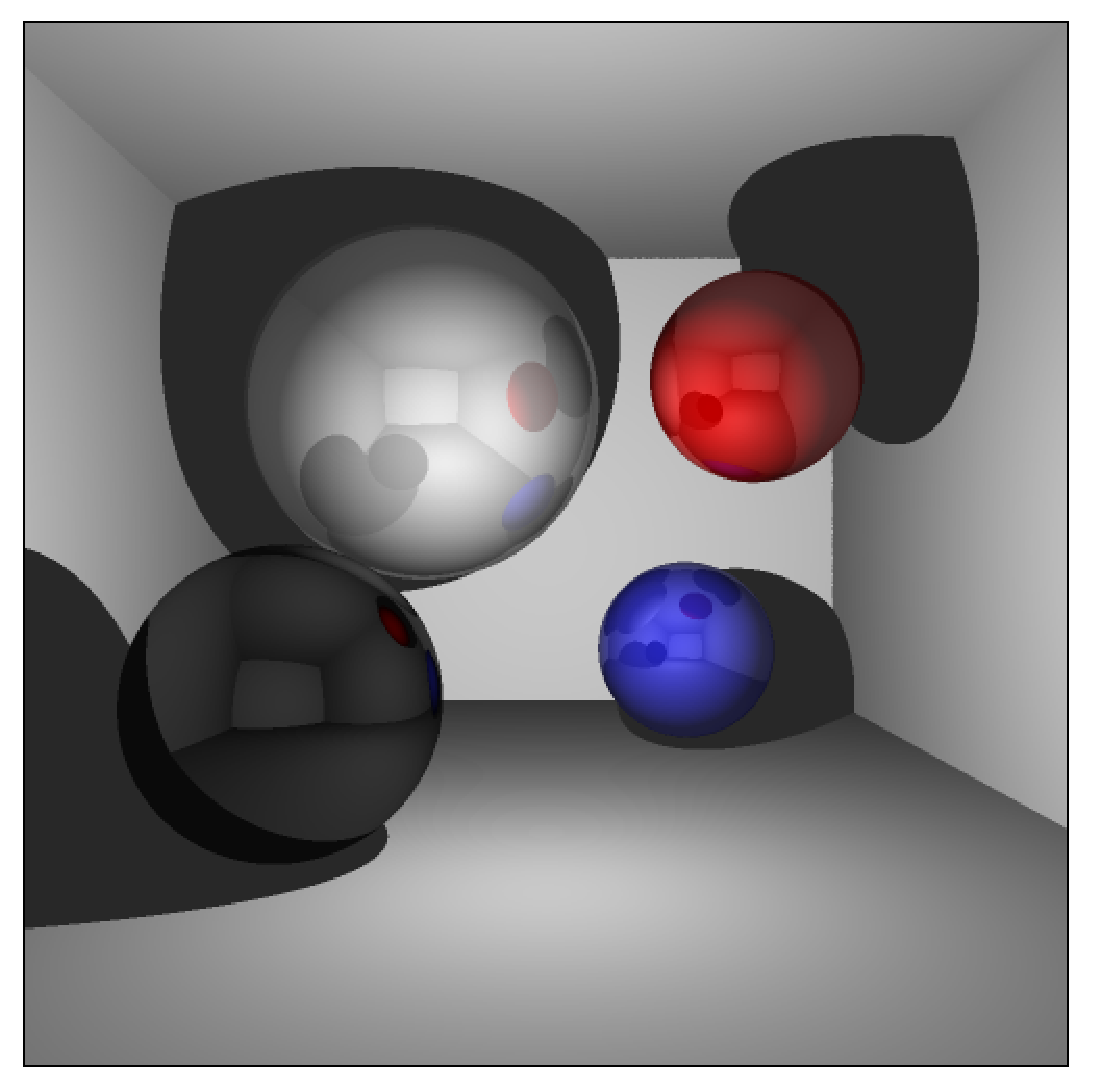
\includegraphics[scale=0.5]{raytracerscreenshot.eps}
\caption{Ray traced 3D scene}
\end{center}
\label{raytracerscreenshot}
\end{figure}

\subsection{Mathematical Underpinnings}
The main objects of operation of the ray tracer are rays given by a position and a normalised direction vector: $r = \langle \vec{p}, \vec{d} \rangle$. It is important to note that rays are unlike lines in that they start at position $\vec{p}$ and only extend in the direction given by $\vec{d}$ whereas lines extend to infinity in both directions.

The ray tracer further includes spheres given by a position and a radius: $s = \langle \vec{p}, r \rangle$. It also includes planes given by its normal and the distance from the origin $p = \langle \vec{n}, d \rangle$ and spotlights simply given by a position vector $l = \vec{p}$.

When tracing a ray $r$, the first step is to find the closest object that intersects the path or $r$ if such an object exists. For this, it is necessary to compute both the intersection point and of a ray with both spheres and planes and also obtain the distance to the object, if there is such an intersection point. We will first describe this computations for a ray and a plane before explaining the more complex computation for a ray and a sphere.

Given the ray $r = \langle \vec{p}, \vec{d_r} \rangle$ and the plane $p = \langle \vec{n}, d_p \rangle$. If the dot product $a$ of the direction vector of the ray and the normal of the plane $\vec{d_r} \cdot \vec{n}$ is equal to $0$, the ray runs parallel to the plane and does not intersect the plane\footnote{Experimental results proved that it is not necessary for successful rendering to consider the case where $r$ lies on the plane.}. If $a \neq 0$ , we treat the ray as a line and calculate $t$, a scalar with the property that $\vec{p} + t*\vec{d_r}$ gives the intersection point of ray and plane. This scalar is given by $-d_p-(\vec{p} \cdot \vec{n}) / (\vec{d_r} \cdot \vec{n})$. If $t < 0$, the plane lies behind the origin of the ray and there is no intersection point of $r$ and $p$.

Calculating the intersection point and $t$ of a ray $r = \langle \vec{p_r}, \vec{d_r} \rangle$ and a sphere $s = \langle \vec{p_s}, r_s \rangle$ is somewhat more complex. The calculation used in the LJSP ray tracer described in the following is mostly based on \cite{physrendering}.

Because the calculations will be made in the object space of $s$, which is the 3D space where the origin lies at $\vec{p_s}$, it is necessary to first translate both $r$ and $s$ to this space. This is very simple in the case of the sphere: Its position is simply set to $(0,0,0)$ as that is how the object space of $s$ is defined. To translate $r$ to the object space of $s$, it is necessary to subtract $\vec{p_s}$ from $\vec{p_r}$. The direction vector of the ray is independent of the position of the ray and does not need to be changed. To make the computation efficient, three temporary variables are now computed that are used repeatedly in the remaining computation:
\begin{equation*}
\begin{aligned}
A &= d_r \cdot d_r\\
B &= 2 \cdot (d_r \cdot p_r)\\
C &= p_r \cdot p_r - r_s \cdot r_s\\
D &= B \cdot B - 4 \cdot A \cdot C
\end{aligned}
\end{equation*}

Calculating the intersection point means solving a quadratic equation that the variable $D$ is the discriminant of. If $D < 0$, the equation has no solution and $r$ and $s$ do not intersect. If $D \geq 0$, two more variables are computed:
\begin{equation*}
\begin{aligned}
t_0 &= \frac{-B-\sqrt{D}}{2 A}\hspace{1.5cm}
t_1 &= \frac{-B+\sqrt{D}}{2 A}
\end{aligned}
\end{equation*}

If both $t_0$ and $t_1$ are less than $0$, there is no intersection point. If one of these two values is less than $0$, the other is returned as $t$. Otherwise the smaller one is returned.

Returning to the process of tracing a ray $r$, after calculating the closest intersection point of the ray with the objects in the scene, the tracing function determines if this intersection point is illuminated by the spot light or if the light is obscured by some other object. It does so by constructing a new ray $r_n = \langle \vec{i}, \vec{d_l} \rangle$ with its position vector $\vec{i}$ being the intersection point and its direction vector $\vec{d_l}$ being a vector going from the intersection point to the light. Again, the closest intersection point of this ray with the objects in the scene is calculated. If there is none, or if it lies behind the light as seen from the ray, the original intersection point is visible from the light, otherwise it is not.

If the point is illumnated by the light, the tracing function next calculates proper shading. If the light from the spot light hights the object that the $r$ intersects with at an angle, the intensity of the light is less than when it hits the object head-on. The intensity of the light hitting the intersection point is calculated by forming the dot product of the objects normal at the intersection point and the direction to the light calculated earlier as $\vec{d_l}$. To imitate ambient light, this value is set to $0.2$, if it is less than that.

If the object hit by the ray $r$ is reflective, the tracing function recurses by tracing the reflection ray before returning a combination of the result of the recursion with the colour of the object. Otherwise it returns the objects colour illuminated with the light calculated in the last section.

\chapter{Implementation}

This chapter will describe the implementation details of the LJSP compiler. It builds on and assumes the previous chapter which describes the parts of the compiler from a theoretical perspective.

We will first give an overview of the code that the LJSP compiler generates, before explaining the structure of the compiler, the implementation of its stages and code emission in one section each. The reason for explaining the generated code first, is that many of the internals of the compiler follow the requirements of the code that it generates. Following this, we give a detailed overview of the implementation of the ray tracer.

\section{Details of the Generated Code}
This section will give a detailed description of the code that the LJSP compiler outputs. It will first describe the asm.js modules generated by the compiler before explaining the C and LLVM code it generates.

\subsection{Asm.js Modules}
\subsubsection{Memory model}
Asm.js offers three ways of saving values to memory: local variables, global variables and a heap in the form of an \texttt{ArrayBuffer}. In the modules generated by the compiler, all these variables are of type double and get casted to integers only inside expressions when necessary.

Local variables are variables local to the function they are declared in. All local variables in a function have to be declared at the top of the function. When the compiler converts an asm.js AST to code, it scans through all functions to find local variables that are used inside the function to create the appropriate declarations. Because all local variables are of type double, all these declarations are of the form \texttt{var n = 0.0;}, because the way to declare a variable as double in asm.js is to initialise it with a floating point value.

Every asm.js module generated by the LJSP compiler has exactly four global variables, shown by the code snipped shown in Fig. \ref{iasmjsmm1}. 
\begin{figure}[ht]
\begin{lstlisting}
var sqrt = stdlib.Math.sqrt;
var floor = stdlib.Math.floor;
var D32 = new stdlib.Float32Array(heap);
var mem_top = 0.0;
\end{lstlisting}
\caption{Global variables of asm.js modules}
\label{iasmjsmm1}
\end{figure}

The first two global variables import two functions to the module: The square root function, which is used to implement the \texttt{sqrt} operator that LJSP includes as to its specification, and the floor function, which rounds a floating point number down to the previous integer. This function is used in the code to convert variables from float to integer.

Global variable \texttt{D32} holds a Float32 View to the heap as explained in the Background Chapter. Because all variables in LJSP are of type double, only this one view to the heap is necessary.

The last global variable, \texttt{mem_top} is used for memory management. This leads to the next section, the memory model used for managing the heap.

After Closure Conversion, the code includes calls to the \texttt{make-env} and \texttt{make-hl} functions that, in conjunction, are used to create closures.  The IR function in the example shown in Fig. \ref{iasmjsmm2} is taken from a program that computes fibonacci numbers (the code was rearranged slightly to make it more readable). Note how the closure created in lines 6 and 7 is not called right away, but instead given as parameters to a recursive call to fib in line 8.

\begin{figure}[ht]
\begin{lstlisting}
function fib(cont, n) {
    if (n < 2.0) {
        cont.code(cont.env, 1.0)
    } else {
        var_3 = n - 1.0
        env = make-env(n, cont)
        closure = make-hl(func_0, env)
        fib(closure, var_3)
    }
}
\end{lstlisting}
\caption{IR code for calling a closure taken from a real example}
\label{iasmjsmm2}
\end{figure}

In asm.js code, this data structure is implemented with arrays that are saved in the \texttt{ArrayBuffer} object. Every asm.js module generated by the LJSP compiler includes a function called alloc shown in Fig. \ref{iasmjsmm3}. This function is used to allocate memory for new arrays.

\begin{figure}[ht]
\begin{lstlisting}
function alloc(size) {
    size = +size;
    var current_mem_top = 0.0;

    current_mem_top = mem_top;
    mem_top = +(mem_top + size);

    return +current_mem_top;
}
\end{lstlisting}
\caption{The \texttt{alloc} function}
\label{iasmjsmm3}
\end{figure}

The \texttt{alloc} function takes the number of needed elements and returns the index to the first element of a subarray of the heap of the required size. The variable \texttt{mem_top} always holds the next element of unallocated memory.

The closure data structure is built by the compiler out of array as follows: It consists of a pointer to an array with two elements. The first element gives the index to the function in one of the function tables that contains the code of the closure. The second element contains a pointer to another array with a variable number of elements that contains the closure's environment. Figure \ref{asmjsclosure} shows this structure.

\begin{figure}[ht]
\begin{center}
\includegraphics{closureasmjs.eps}
\end{center}
\caption{The closure data structure in asm.js code}
\label{asmjsclosure}
\end{figure}


Because this variable gets increased by every memory allocation, it is necessary to free memory somewhere in the code, if we want to avoid memory overflows. The place where this happens are the functions that end in \texttt{_copy}, introduced by CPS-translation. Because the functions are the entry points to the module, they reset \texttt{mem_top} to $0$ before calling the function they were copied from. This is possible because in LJSP, no state is shared between function calls.

The example shown in Fig. \ref{iasmjsmm4} shows the asm.js code of the \texttt{_copy} function for the \texttt{fib} function from the example above. Detailed explanations of all statements will be given in the next section.

\begin{figure}[ht]
\begin{lstlisting}
function fib_copy(n){
// Parameter n is of type double
n = +n;

// Declare vars
var closure = 0.0, env = 0.0;

// Reset memory
mem_top = 0.0;

// Create continuation closure
env = +alloc(+0);
closure = +alloc(+2);
D32[(~~+floor(+(closure + 0.0))|0) << 2 >> 2] = 2.0;
D32[(~~+floor(+(closure + 1.0))|0) << 2 >> 2] = env;

// Call original function
return +fib(closure, n);
}
\end{lstlisting}
\caption{A \texttt{_copy} function}
\label{iasmjsmm4}
\end{figure}

This example also illustrates why \texttt{_copy} functions are necessary. Memory management is internal to the module and can not be accessed by the code calling functions inside the module. It would therefore be impossible for the caller to create the continuation that the \texttt{fib} function takes as it first argument and that \texttt{fib_copy} creates in lines 11 to 14.

\subsubsection{Structure of the Module}

Asm.js modules generated by the LJSP compiler are made up of the following elements:
\begin{itemize}
\item The four global variables and the \texttt{alloc} function that were described in the previous section
\item A number of functions
\item A number of function tables
\item A return statement
\end{itemize}

An example return statement from the gen_code.js file included in the repository is given in Fig. \ref{iasmjsmm5}. Only the \texttt{_copy} functions are exported from the module to ensure that only these functions are used as entry points and the heap gets properly reset before every computation. They are, however, exported under their original name (without the suffix), which makes the copying completely transparent to the user.

\begin{figure}[ht]
\begin{lstlisting}
return {vectorsDotProduct: vectorsDotProduct_copy, 
    raySphereIntersectionPoint: 
    raySphereIntersectionPoint_copy};
\end{lstlisting}
\caption{The return statement of a real asm.js module}
\label{iasmjsmm5}
\end{figure}

The function tables of the same program are shown in Fig. \ref{iasmjsmm6}. All functions in the module can be found in one of the function tables, even if they are always called by name. The name assigned to every table consists of \texttt{ftable} followed by the number of parameters the functions in that table take. This is visible in the fact that \texttt{_copy} functions can always be found in a function table with a parameter count one less than the table that contains the original function. In the example below, \texttt{vectorsDotProduct_copy} is in \texttt{ftable6} and \texttt{vectorsDotProduct} is in \texttt{ftable7}.

As mentioned in the Background Chapter, every function table has to have a size equal to a power of two. Because it is not always the case that this matches with the number of functions in the module, function tables with a length not equal to $2^x$ have their size increased to the next higher power of two by appending the first function in the table as many times as necessary. An example of this is \texttt{ftable2} in the code, which had its first element copied three times to reach a size of $2^3$. These copied functions are not used and only necessary to create valid asm.js code.

\begin{figure}[t]
\begin{lstlisting}
var ftable6 = [vectorsDotProduct_copy];
var ftable7 = [vectorsDotProduct];
var ftable2 = [func_0, func_1, func_2, func_3, func_4,
               func_0, func_0, func_0];
var ftable10 = [raySphereIntersectionPoint_copy];
var ftable11 = [raySphereIntersectionPoint];
\end{lstlisting}
\caption{Function tables in asm.js}
\label{iasmjsmm6}
\end{figure}

To conclude this section, we will describe some of the more complex statements that the compiler outputs.

While heap assignments work in principle as described above, in practise they require a number of casts and type coercions that makes them quite hard to read. The short example given in Fig. \ref{iasmjsmm7} shows the creation of a closure. Except for line breaks, variable renaming and the removal of redundant parentheses, this is unedited asm.js code as generated by the compiler.

\begin{figure}[ht]
\begin{lstlisting}
env = +alloc(+4);
D32[(~~+floor(+(env+0.0))|0) << 2 >> 2] = A;
D32[(~~+floor(+(env+(1.0))|0) << 2 >> 2] = cont_1;
D32[(~~+floor(+(env+2.0))|0) << 2 >> 2] = s_r;
D32[(~~+floor(+(env+(3.0))|0) << 2 >> 2] = var_28;
closure = +alloc(+2);
D32[(~~+floor(+(closure+0.0))|0) << 2 >> 2] = 2.0;
D32[(~~+floor(+(closure+1.0))|0) << 2 >> 2] = env;
\end{lstlisting}
\caption{Creating a closure in asm.js}
\label{iasmjsmm7}
\end{figure}

Creating a closure entails first creating the environment and then creating the closure itself. In the code above, the environment is created in lines 1 to 5. Because it is made up of four variables, the first line allocates an array with four elements. The \texttt{+} signs in front of the call to \texttt{alloc} and many other expressions in the code are type coercions. These are explained in detail in the Background Chapter.

After allocating memory in line 1, the four variables that make up the environment (\texttt{A}, \texttt{cont_1}, \texttt{s_r} and \texttt{var_28}) are assigned to the four spaces in the array in lines 2 to 5. The computation of the index to \texttt{D32} consists of many different parts that we will now go through in detail.

The expression \texttt{... {<}< 2 {>}> 2} on the very outside does not change the result of what comes before it, but is necessary because the asm.js spec requires a right shift by $log_2~4$ when accessing the heap through a view with a datatype of length four bytes such as Float32Array. Because this right shift on its own would change the value of the index we compute, we add a left shift by the same number of bits in front of the right shift. This problem could also be solved by changing array index computation so that the right shift alone computes the correct result, but in practise, this back and forth shifting turned out to have a small impact on performance.

The remaining expression is a call to the floor function of the following, somewhat odd looking, form: \texttt{\textasciitilde\textasciitilde+floor(...)|0}. This is the asm.js way of casting a double to an integer. This is necessary, because all variables in the module are of type double, but array indices have to be of type int. This typecasting could be avoided by making parameters and variables that are used as indices to access the heap of type int instead of double. Because all functions in one function table have to have the same type signature, however, this would require complex changes to the compiler and is left as future work. Inside that cast, the variable holding the base of the environment (\texttt{env}) is added to an offset going from $0$ to $3$. 

After the environment variable has been constructed, the rest of the example creates the closure itself. As mentioned above, closure variables are arrays of length two. In line 7, the index to the function in its function table is assigned to the element at offset 0. Line 8 assignes the environment variable to the element at offset 1.

While the number assigned in line 7 seems, at first sight, to give insufficient information to identify the function to be called as there is more than one function table in the program, it does, in fact, suffice to uniquely determine the correct function table the index belongs to. The reason for this is that later in the code when this closure is called, the number of parameters it is called with, is known at compile time. The name of the function table is then given by the expression \texttt{"ftable" + (params.size + 1).toString}, because function tables are named after the number of paramters the functions they contain take.


\subsection{C Code}
\subsubsection{Memory model}
Unlike asm.js, which uses global variables, the C code only use local variables and memory on the heap allocated with \texttt{malloc}. While in asm.js modules, functions take parameters of type double, in the C code, all parameters are pointers of type \texttt{void*}. The reason for this is that both pointers to double values and arrays are passed to the function through its parameters. Based in what context the parameters are used inside the function, they are cast to the appropriate type and dereferenced.

This means that it is not possible to pass static double values as arguments to function calls. Instead, it is necessary to allocate memory on the heap, write the value to that allocated space in memory and pass a pointer to it in the function call. An example of this is given in Fig. \ref{icmm1}.

\begin{figure}[ht]
\begin{lstlisting}
const_0 = (double*)malloc(sizeof(double) * 1);
*const_0 = 1000000.0;
ret_val_3 = func_pointer_0(env_param_0, const_0);
\end{lstlisting}
\caption{Calling a function with a static value as parameter}
\label{icmm1}
\end{figure}

To make it possible to pass local variables as arguments to functions, they are declared to be of type \texttt{double*}, assigned memory allocated with \texttt{malloc} and dereferenced when read from or written to. Simply passing a reference in a function call would lead to a crash as local variables are allocated on the stack and destroyed when the function they are local to returns.

Creating closures is done simmilarly to asm.js code. Figure \ref{icmm2} shows the C version of the code given in Fig. \ref{iasmjsmm7}.

\begin{figure}[ht]
\begin{lstlisting}
env = (void**)malloc(sizeof(void*) * 4);
env[0] = A;
env[1] = cont_1;
env[2] = s_r;
env[3] = var_28;
closure = (void**)malloc(sizeof(void*) * 2);
closure[0] = &func_2;
closure[1] = env;
\end{lstlisting}
\caption{Creating a closure in C}
\label{icmm2}
\end{figure}

The major difference between asm.js and C is that in the C code above, \texttt{closure[0]} is assigned a function pointer to the function to be called as there are no function tables in C. Calling a closure is slightly more complex than creating it. Figure \ref{icmm3} shows how a closure is called in C.

\begin{figure}[ht]
\begin{lstlisting}
// Variable declarations
void** casted_hl_var_0;
void* uncast_func_pointer_0;
void *(*func_pointer_0)(void*,void*);
void* env_param_0;
double* const_0;

...

// Calling cont_1
casted_hl_var_0 = (void**)cont_1;
uncast_func_pointer_0 = casted_hl_var_0[0];
func_pointer_0 = 
    (void* (*)(void*,void*))uncast_func_pointer_0;
env_param_0 = casted_hl_var_0[1];
const_0 = (double*)malloc(sizeof(double) * 1);
*const_0 = 1000000.0;
ret_val_3 = func_pointer_0(env_param_0, const_0);
\end{lstlisting}
\caption{Calling a closure in C}
\label{icmm3}
\end{figure}

Lines 11 to 15 are casts and assignments to obtain the function pointer and the environment variable from the closure. Line 16 and 17 were described in the first example of this section. Line 18 is the function call itself.

Figure \ref{cclosure} shows the closure data structure used in C code. It is quite similar to the asm.js data structure shown in Figure \ref{asmjsclosure}. The first difference between the two is that in the generated C code, the first element of the closure data structure points directly to a function as opposed to giving an index for a function table. The second difference is that in the environment array in C code is made up of pointers to double values, whereas in asm.js the environment array contains the values themselves.

\begin{figure}[ht]
\begin{center}
\includegraphics{closurec.eps}
\end{center}
\caption{The closure data structure in C code}
\label{cclosure}
\end{figure}

Although this structure is equal for all closures used in the generated C code, it always constructed ad-hoc with calls to \texttt{malloc}, casts and array accesses instead of using a C-style \texttt{struct}. While this could change in the future, readability of the code that the LJSP compiler generates was not a design goal during its development.

Before concluding this section, there is one remaining aspect of memory management in C worth mentioning. The C code genreated by the "Conversion to C" stage is designed to run as an executable and terminate after computing and outputting the result of the expression given together with the \texttt{define}s. C code generated by "Conversion to Emscripten C" however does not terminate but instead keeps running and has its functions called many times. This makes it necessary to free memory allocated by the functions if an overflow is to be avoided. The way this is achieved is by implementing a custom memory manager. This memory manager can be found in the file \texttt{jalloc.c} and includes two functions: \texttt{jalloc}, which replaced \texttt{malloc} and \texttt{free_all}, which frees all the memory allocated with \texttt{jalloc}. Like in the asm.js modules, the entry point functions ending in \texttt{_copy} reset the memory before calling the function they were copied from.

\texttt{jalloc} is implemented using a linked list. Every block of memory requested is added as a node to the list before being returned. The \texttt{free_all} function goes through this list from head to tail and calls \texttt{free} on all memory saved in it.

\subsubsection{Structure of the Module}
C code as generated by the LJSP compiler is made up of three sections:
\begin{itemize}
\item Preprocessor directives
\item Function declarations
\item Functions
\end{itemize}

The preprocessor directives are the same for all programs and are shown in Fig. \ref{icmm4}.

\begin{figure}[ht]
\begin{lstlisting}
#include <stdio.h>
#include <stdlib.h>
#include <math.h>
    
#define min(x,y) ((x)<(y)?(x):(y))
#define max(x,y) ((x)>(y)?(x):(y))
\end{lstlisting}
\caption{Preprocessor direcives used in compiled C code}
\label{icmm4}
\end{figure}

\texttt{stdio.h} is included to be able to print the result of the program to the command line, \texttt{stdlib.h} provides the \texttt{malloc} function used to allocate memory and including \texttt{math.h} is necessary to be able to use the \texttt{sqrt} function to calculate square roots. The \texttt{min} and \texttt{max} functions are implemented using the tertiary operator.

The function declarations include all functions in the file except \texttt{main}, so that they can call each other and don't need to be defined in a particular order.

The function block includes all the function that are present in IR code before the "Conversion to C" stage. It further includes a new function introduced by this stage called \texttt{expression} which takes no parameter and has as its body the expression of the program. It also includes a \texttt{main} function, shown in Fig. \ref{icmm5}, which calls the \texttt{expression} function and prints its result to the console.

\begin{figure}[ht]
\begin{lstlisting}
int main(int argc, char **argv) {
    double *r = expression();
    printf("%f\n", *r);
}
\end{lstlisting}
\caption{The main function used in compiled C code}
\label{icmm5}
\end{figure}

The functions themselves are split into a set of variable declarations and a list of statements. Generally, the statements are quite similar to IR code. One noteworthy exception are primitive operations which are much more complex, as these operations are performed on void pointers and the result must be written to a double pointer. The example given in Fig. \ref{icmm6} shows the result of converting the IR statement \texttt{var_2 + var_4} to C:

\begin{figure}[ht]
\begin{lstlisting}
prim_op_p_1 = (double*)var_2;
prim_op_v_1 = *prim_op_p_1;
prim_op_p_2 = (double*)var_4;
prim_op_v_2 = *prim_op_p_2;
var_1 = (double*)malloc(sizeof(double) * 1);
*var_1 = prim_op_v_1+prim_op_v_2;
\end{lstlisting}
\caption{A primitive operation in C}
\label{icmm6}
\end{figure}

Both operands are first cast from a \texttt{void*} to a \texttt{double*}, before getting dereferenced. The result, i.e. the values to be added are then saved in two variables (\texttt{prim_op_v_1} and \texttt{prim_op_v_2} in the example). Before the addition takes place, memory is allocated to hold the result and assigned to a \texttt{double*}. In the last line, the sum of the two operands is then written to the memory allocated in the previous line.

As mentioned in the section on the memory layout of the C code generated by the compiler, there are a few small differences between the code that the "Conversion to C" stage and the "Conversion to Emscripten C" emit. "Conversion to Emscripten C" removes the \texttt{expression} and \texttt{main} functions. They are unnecessary, because Emscripten compiles the C code to an asm.js module which will have its functions called by some other piece of code. "Conversion to Emscripten C" further replaces calls to \texttt{malloc} to \texttt{jalloc} and adds a call to \texttt{free_all} to \texttt{_copy} functions, as mentioned above, and adds the line \texttt{\#include "jalloc.c"} to the preprocessor block to make this function available. The last change it makes is adding another copy of every function that ends in \texttt{_copy} with the suffix \texttt{_call_by_value}. These new functions take the same number of parameters as the original functions, but their parameters are of type \texttt{double} instead of \texttt{double*}. This is necessary for the same reason the \texttt{_copy} functions are necessary for: The calling code has no access to the memory handling of the module that Emscripten generates and can not allocate any memory that the double pointers could point to. This is instead done by the new \texttt{_call_by_value} functions.

\section{Structure of the Compiler}
The LJSP compiler itself is written in Scala and spread out over a number of files. The code of the compiler follows a logical structure that separates the code into modules and that makes it easy to find related modules. The necessity for a clear structure became evident quickly during the development of the compiler, as it was often necessary to edit multiple parts of the code simultaneously.

The code is structured as follows:
\begin{itemize}
\item The entry point of the compiler can be found in \texttt{main.scala}. This files contains functionality to parse and dispatch the arguments the LJSP compiler gets called with by calling the appropriate methods to achieve the desired result.
\item All classes that make up the Abstract Syntax tree can be found in \texttt{AST.scala}. We decided against splitting up this file into a separate file for each language used in the LJSP compiler (LJSP, IR, C, etc.) as that would have lead to unnecessary fragmentation.
\item The compilation stages that make up the LJSP compiler can be found in files with file names starting with a number, e.g. \texttt{03_cps_translation.scala}, optionally followed by a letter that gives a hint as to which stages precede and follow it. These files all contain exactly one object with a name equal to the file name without the number (\texttt{object cps_translation} in the example of CPS-translation) which in turn contain all the methods used in conversion. 
\item The functions that convert ASTs back to specific languages can be found in files that have file names starting with \texttt{code_generation_}. There are five such files in total, one each for every programming language that the LJSP compiler converts to or from: LJSP, IR, asm.js, C and LLVM IR.
\item The file \texttt{run_tests.py} contains the testing framework described further down in the Testing Chapter. All other files related to testing can be found in the \texttt{test/} folder.
\item The ray tracer and all files related to it reside in the \texttt{ray_tracer/} folder.
\item \texttt{jalloc.c} contains a custom memory mananger that will be explain in the next section.
\item The file \texttt{util.scala} contains a small number of utility functions used throughout the rest of the code.
\end{itemize}

\section{Implemenation of Various Stages}
This section will describe the implementation details of most stages. The stages not mentioned in this section follow the theoretical description given in the Design Chapter so closely that there is nothing that stands out enough to warrant inclusion in this chapter.
\subsection{Parsing}
Parsing is implemented using the parser combinator classes of the Scala standard library. This makes the code terse and readable. Because LISP is a very easy language to parse, writing a custom parser for LJSP would not have yielded very interesting results. We therefore decided against implementing our own parsing library. The parser clearly reflects the grammar of LJSP in code form. The grammar rule for a \texttt{define} is given in the Specification Chapter as follows:

\begin{grammar}
<define> ::= `(define (' <ident> <params> `)' <expr> `)'

<params> ::= <ident> <params> | $\epsilon$
\end{grammar}

This rule is still visible in the Scala. Note that for the Scala parser combinators, \texttt{rep} has the meaning of "Zero or more", which made the additional \textit{params} rule unnecessary in the code. The parsing rule for \texttt{define}s is shown in Fig. \ref{parsingrule}.

\begin{figure}[ht]
\begin{lstlisting}
def define: Parser[SDefine] = 
"(" ~> "define" ~> "(" ~> 
    identifier ~ rep(identifier) ~ ")" ~ 
    expression <~ ")" ^^ {
        case name~params~")"~e => 
            SDefine(name, params, e)
}
\end{lstlisting}
\caption{The parsing rule for \texttt{define}s}
\label{parsingrule}
\end{figure}


\subsection{Prim op reduction}
After the completion of this stage, the following primitive operations will have been removed: 
\begin{itemize}
\item The arithmetic negation operator \texttt{neg}. In most other languages, \texttt{-} is used for this. This operator is reduced to a subtraction from zero; the expression \texttt{(neg x)} gets converted to \texttt{(- 0 x)}.
\item The boolean negation operator \texttt{not}. This is often written as \texttt{!} in computer science or $\neg$ in mathematics. If-expressions of the form \texttt{(if (not $e_1$) $e_2$ $e_3$)} have their true and false branch swapped and get reduced to \texttt{(if $e_1$ $e_3$ $e_2$)}.
\item The boolean \texttt{and}. Expressions of the form \texttt{(if (and $e_1$ $e_2$) $e_3$ $e_4$)} are converted to two nested if-expressions: \texttt{(if $e_1$ (if $e_2$ $e_3$ $e_4$) $e_4$)}
\item The boolean \texttt{or}: If-expressions of the form \texttt{(if (or $e_1$ $e_2$) $e_3$ $e_4$)} get converted to two nested if-expressions: \texttt{(if $e_1$ $e_3$ (if $e_2$ $e_3$ $e_4$))}, analoguously to \texttt{and} conversion
\item \texttt{>=}. Expressions of the form \texttt{(>= $e_1$ $e_2$)} are reduced to the expression \texttt{(not (< $e_1$ $e_2$))} which then gets reduced recursively according to the rule to remove \texttt{not}s explained above.
\item \texttt{<=}, equivalent to \texttt{>=} above.
\end{itemize}

\subsection{CPS-Translation}
The code for CPS-translation closely resembles the equations given in the Design Chapter. One peculiarity of the CPS-translation function is that it comes in two versions taking two different types of continuations. The first line of the definitions of both functions are shown in Fig. \ref{cpstranstwofuncs}.

\begin{figure}[ht]
\begin{lstlisting}
def cps_trans(e: SExp, k: SExp => SExp) : SExp
def cps_tail_trans(e: SExp, c: SExp) : SExp
\end{lstlisting}
\caption{The two functions that CPS-translate LJSP expressions}
\label{cpstranstwofuncs}
\end{figure}

While both function take the expression to be CPS translated as their first parameter, the first function takes a function that maps an \texttt{SExp} to an \texttt{SExp} as its second parameter while the second function takes the continuation in a simple \texttt{SExp}. In effect, the first function takes a part of the Abstract syntax tree that the result of CPS-Translating \texttt{e} is to be inserted into, while the second function takes an expression that contains the continuation in the context of the program to be compiled.

To further illustrate this concept, consider the translation of \texttt{SIf} statements used in earlier versions of the compiler shown in Fig. \ref{ifcpstrans}.

\begin{figure}[ht]
\begin{lstlisting}
case SIf(e1, e2, e3) => {
    val c = SIdn(fresh("var"))
    val p = SIdn(fresh("var"))
    
    cps_trans(e1, (ce1: SExp) =>
        SLet(c, SLambda(List(p), k(p)),
            SIf(ce1, cps_tail_trans(e2, c), 
                     cps_tail_trans(e3, c))))}
\end{lstlisting}
\caption{\texttt{if}-tranlsation rule used in early versions}
\label{ifcpstrans}
\end{figure}

In the mathematical notation used in the Design Chapter, this can be expressed as:

\begin{alignat*}{2}
&\cpstrans{(\text{if}\ e_1\ e_2\ e_3)} k &&\eqdef \cpstrans{e_1} \lambda x.(\text{let}~c~=~\lambda p.k(p)~\text{in}~(\text{if}\ x\ \cpstrans{e_2}c\ \cpstrans{e_3}c) \\
\end{alignat*}

This version of the CPS-translation of if-expressions creates a lambda ($\lambda p.k(p)$ in the equation above) and CPS-translates $e_2$ and $e_3$ with this lambda as their continuation. Because this is a lambda in the context of the program, not in the context of the compiler, it requires the additional \texttt{cps_tail_trans} function.

In contrast, the CPS-translation of if-expressions in the current version of the compiler is shown in Fig. \ref{ifcpstranscurrent}.

\begin{figure}[ht]
\begin{lstlisting}
case SIf(e1, e2, e3) => {
    cps_trans(e1, (ce1: SExp) => 
        SIf(ce1, cps_trans(e2, k), 
                 cps_trans(e3, k)))}
\end{lstlisting}
\caption{\texttt{if}-tranlsation rule used in current versions}
\label{ifcpstranscurrent}
\end{figure}

Or expressed in mathematical notation:

\begin{alignat*}{2}
&\cpstrans{(\text{if}\ e_1\ e_2\ e_3)} k &&\eqdef \cpstrans{e_1} \lambda x.(\text{if}\ x\ \cpstrans{e_2}k\ \cpstrans{e_3}k) \\
\end{alignat*}

This version applies the continuation function k twice. This avoids the introduction of the \texttt{lambda} necessary in the previous version, but comes at the cost of code duplication: The AST subtree saved in k will be used in both branches of the if-expression. We will return to this trade off in the Evaluation Chapter where the reasoning behind the choice for the second version will be explained. It is, however, important to mention here that \texttt{cps_tail_trans} can not be avoided completely: When CPS-translating \texttt{SDefine} and \texttt{SLambda}-expressions that receive their continuations in a parameter, it is necessary to use \texttt{cps_tail_trans}, as these parameters are again on the level of the program, not on the one of the compiler.


\subsection{Hoisting}
The hoisting transformation makes use of an internal class named \texttt{HoistedExpression}. This class is used to accumulate hoisted functions when recursively traversing the Abstract Syntax Tree.

In earlier versions of the compiler, this was implemented using Scala tuples, but using a dedicated class was found to improve readability. 


\subsection{Redundant Assignment Removal}
This stage is implemented in a purely functional way. The core of redundant assignment removal is given in slightly edited form in Fig. \ref{remredasign1}.

\begin{figure}[ht]
\begin{lstlisting}
def convert_statements_to_rra_ir(statements: 
                                 List[IStatement]) : 
             List[IStatement] = statements match {
 case Nil => Nil
 case (s::sts) => s match {
  case IVarAssignment(lh, IIdn(rh)) => {
   convert_statements_to_rra_ir(
    sts.map{rename_var_in_ir_statement(_, lh, rh)})
  case _ => s :: convert_statements_to_rra_ir(sts)
 }
}
\end{lstlisting}
\caption{Removing redundant assignments}
\label{remredasign1}
\end{figure}

% TODO LIB better explanation, maybe also pseudocode
This function calls itself recursively for each element in the list, discarding it if it is a redundant assignment and renaming the variable on the left hand side in those cases.

\subsection{Conversion to asm.js}
Besides the rather simple task of converting IR AST classes to their equivalent in the asm.js AST class hierarchy (\texttt{IStaticValue} to \texttt{AStaticValue}, \texttt{IFunctionCallByName} to \texttt{AFunctionCallByName}, etc.), this stage makes a number of other major changes to the code.

The first is the generation of function tables. The part of the code that accomplishes is given in Fig. \ref{iconvasmjs1}, again slightly edited.

\begin{figure}[ht]
\begin{lstlisting}
val fs_map = functions.groupBy(_.params.size)

val fnames_map = fs_map.map{ case (size, fs) => 
  ("ftable"+size.toString, fs.map{_.name})}
  
val fnames_map_pow_2 = fnames_map.map{ 
  case (ftable, fnames) => {
  val size_difference = 
    find_next_power_of_2(fnames.size) - fnames.size
  (ftable, fnames ++ 
    List.fill(size_difference)(fnames(0)))
  }
}
\end{lstlisting}
\caption{Creating function tables}
\label{iconvasmjs1}
\end{figure}

The statement in line 1 groups the functions in the \texttt{functions} list by the number of their parameters, creating a Map object that maps parameter count to a list of function objects.

In line 3 and 4, this Map is turned into a second map, now mapping strings of the form \texttt{"ftable2"} to lists of function names.

Finally, the statement spanning from line 6 to 13 goes through every function table, represented by a key/value pair in the map, calculates the difference in the count of function names to the next power of two and fills up the list with enough copies of the first function to reach that next power of two. It does so using the \texttt{fill} method of Scala's \texttt{List} class. This method takes a number \texttt{n} and an object \texttt{o} and creates a list with \texttt{n} copies of \texttt{o}.

After the function tables have been created in such a way, converting a call to a variable holding the index to a function is a simple process. The code that does this is shown in Fig. \ref{iconvasmjs2}. Note how the correct function table name is found simply by adding the number of parameters (increased by one for the environment parameter) to the string \texttt{"ftable"}.

\begin{figure}[ht]
\begin{lstlisting}
case IFunctionCallByVar(hl_var, params) => {
  val converted_params = params.map{
    convert_expression_to_asmjs(ftables, _)}
    
  val ftable_name = 
    "ftable" + (params.size + 1).toString
    
  AFunctionCallByIndex(ftable_name, hl_var, 
                       converted_params)
}
\end{lstlisting}
\caption{Converting calling function variable to asm.js}
\label{iconvasmjs2}
\end{figure}

The third part to calling functions using function tables in asm.js is finding the correct index to the function table determined in the code snipped above. This is done when expanding IR \texttt{make-hl}-expressions to asm.js code that allocates memory and creates the closure. The code for that makes use of a function called \texttt{fname_to_ftable_index} that goes through all function tables and returns the index of the function in the function table it is in.

Finally, this stage introduces return statements to all functions. If the last statement in the function is an expression, that expression is returned. If, however, the last statement is an \texttt{if}-statement, a variable is created that is assigned the last expression of both if-branches and returned after the if statement\footnote{The simpler solution of returning inside the if-branches does not conform to the asm.js specification.}

\subsection{Conversion to C}
This is one of the most complex stages in the LJSP compiler. This is reflected in its implementation, which is long and complex compared to the other stages.

Unlike the other stages, which convert statements of one kind to statements of another kind, this stage converts IR statements to tuples of declarations and C statemnets. This is reflected in the type of the conversion function which returns a result of type \texttt{(List[CDeclareVar], List[CStatement])}. Deriving the correct type of the variables to be declared is one part of the work of this stage.

In the Intermediate Representation, it is not necessary to declare any variables before using them. Consider an IR statement such as \texttt{a = 3.0;}. In C, this statement gets expanded to the code shown in Fig. \ref{iconvc1}.
\begin{figure}[ht]
\begin{lstlisting}
double* a;
...
a = (double*)malloc(sizeof(double) * 1);
*a = 3.0;
\end{lstlisting}
\caption{Converting a simple assignment to C}
\label{iconvc1}
\end{figure}

The implementation of the part of the code that accomplishes this transformation is given in Fig. \ref{iconvc2}.

\begin{figure}[ht]
\begin{lstlisting}
case IVarAssignment(idn, IStaticValue(d)) => {
  (CDeclareVar(idn, CTDoublePointer) :: Nil,
  
  CVarAssignment(idn, 
    Malloc(CTDoublePointer, CTDouble, 1)) ::
  CDereferencedVarAssignment(idn, 
    CStaticValue(d)) :: Nil)
}
\end{lstlisting}
\caption{Converting assignments of static values to C}
\label{iconvc2}
\end{figure}

Line 2 of this example creates the first list in the tuple: a list with one element which contains the declaration of the variable assigned to to be of type \texttt{CTDoublePointer} which is the compiler's representation of \texttt{double*}.

Lines 4 to 7 create the second list of the tuple consisting of the two statements that allocate memory and assign the static value \texttt{d} to the newly allocated memory by dereferencing the variable.

% TODO LIB list types for all expressions:
%iif
%v = a[i]
%fname(p1, p2)
%var(p1, p2)
%v = 3
%v = a + b
%env = make-env
%hl = make-hl
%v1 = v2
%idn
%3


\subsection{Conversion to LLVM IR}

Although the file containing this stage is the largest of all the files containing the compilation stages, this is is a simple stage in terms of the its transformation. Its main function expands every \texttt{CStatement} into a number of LLVM IR statements but it makes no structural changes to the Abstract Syntax Tree.

% TODO LIB give expansions for all C statements



\section{Code Generation}
Generating or emitting code in text form is the reverse of parsing. It's the process of taking an Abstract Syntax Tree and converting it to the textual representation of the programming language. Because of this relationship between parsing and code generation, the latter is sometimes called "unparsing" \cite{nanopass}.

In early versions of the LJSP compiler this was accomplished by simply adding a \texttt{toString} method to all classes that make up the AST. Because converting an expression or statement to a string involves converting all sub-expressions to strings, the \texttt{toString} method of the root object would recursively traverse the entire tree. This lead to very hard to read code. 

It later turned out to be a much better decision to move these code emitting functions to separate files, as described in the section "Structure of the Compiler". These files contain functions that work very similarly to the \texttt{toString} methods used previously in that they recursively traverse the AST, but they are separate from the definition of the class hierarchy in \texttt{AST.scala}.

\section{Implementation Details of the Ray Tracer}
This section will describe the internals of the ray tracer that is included with LJSP.
\subsection{Files Related to Ray Tracing}
All files related to it can be found in the \texttt{ray_tracer/} directory. They are:
\begin{itemize}
\item \texttt{ray_tracer.html}, this is the html file that loads all the JavaScript files and shows a canvas for them to draw on together with four buttons that let the user decide how to render the scene
\item \texttt{ray_tracer.js}, this file contains the ray tracer itself
\item \texttt{ljsp_code.scm}, this file contains an implementation of \texttt{raySphereIntersectionPoint} and \texttt{vectorsDotProduct} in LJSP
\item The remaining JavaScript files contain different versions of the two functions defined in \texttt{ljsp_code.scm} and are explained in detail below
\end{itemize}


\subsection{The HTML Interface}
The user interacts with the ray tracer using the web page contained in\texttt{ray_tracer.html}. This html interface includes a canvas on which the rendered 3D scene will be drawn, four buttons that offer the user a choice of rendering methods as well as a way to display the time it took to render the image. Figure \ref{raytracinginterface} shows this html interface.

\begin{figure}[p]
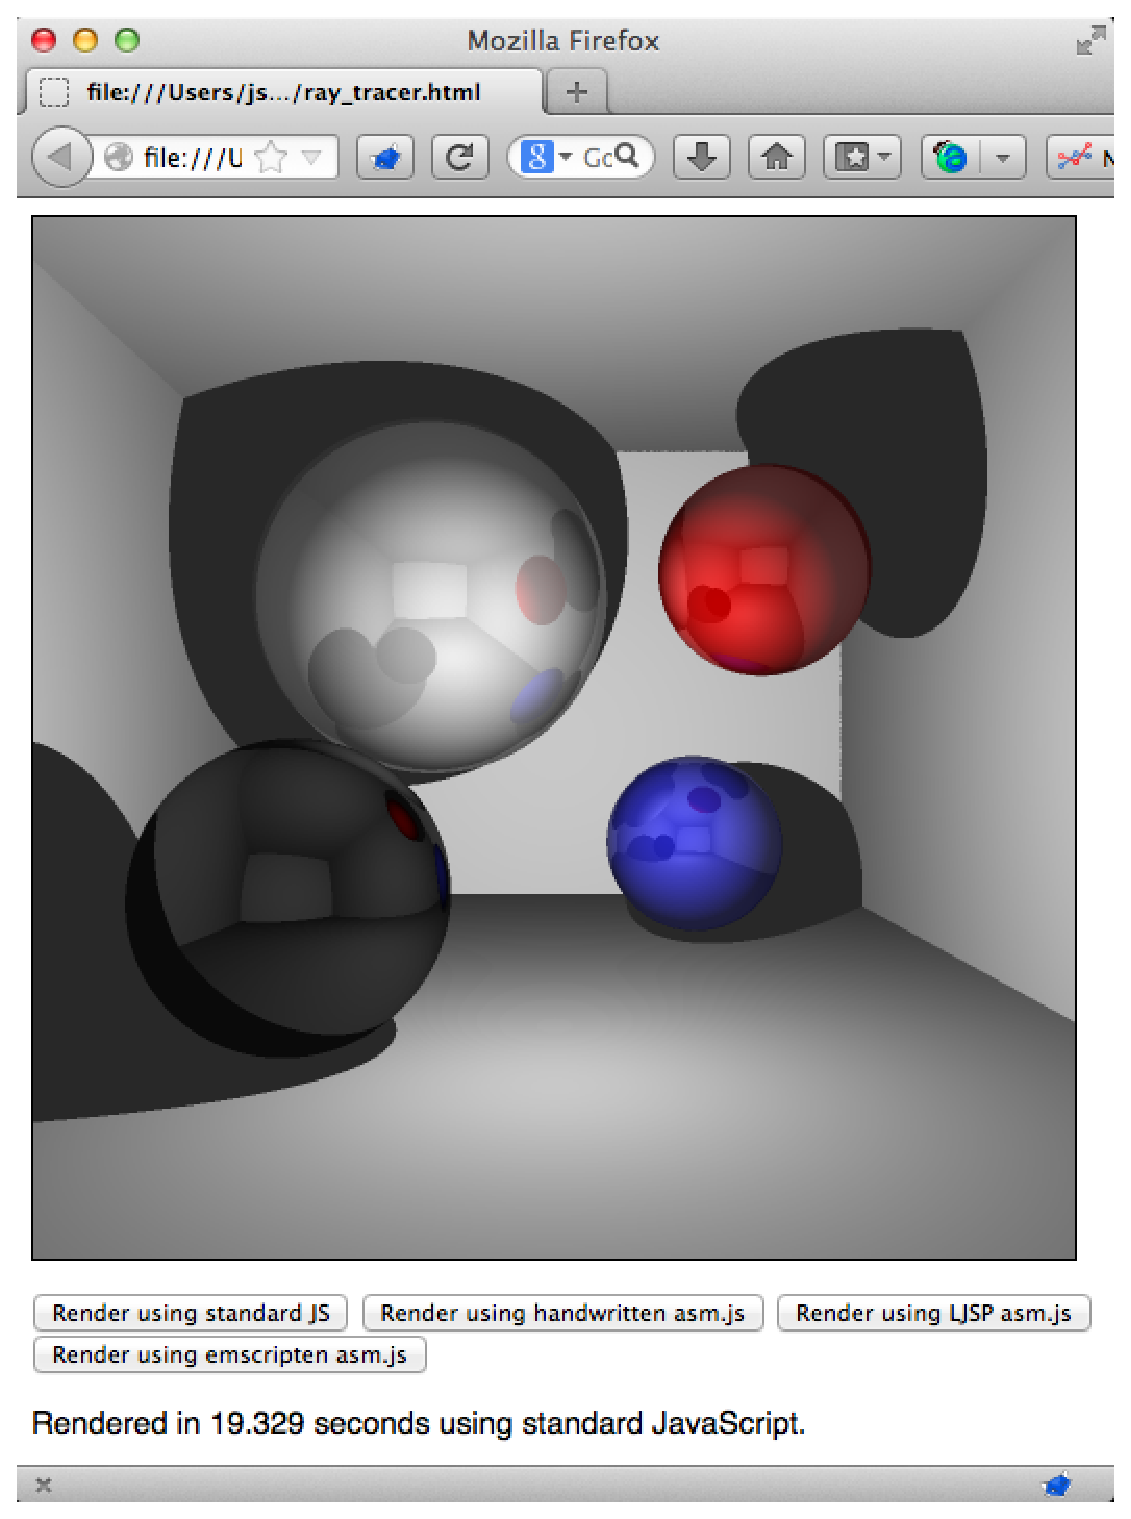
\includegraphics[scale=0.7]{raytracinginterface.eps}
\caption{The ray tracer interface}
\label{raytracinginterface}
\end{figure}

Every rendering method consists of a different implementation of one of the main functions the renderer uses: \texttt{raySphereIntersectionPoint}. This function computes the intersection point of a ray with a sphere. Comparing the running time of the different methods against each other offers a benchmark for each method.

There are four different rendering methods in total which correspond to the four buttons on the html page:

\begin{enumerate}
\item Standard JavaScript, the implementation of this method can be found in the \texttt{ray_tracer.js} file
\item Handwritten asm.js code, this is implemented in \texttt{handwritten_asm.js}
\item Asm.js code generated by the LJSP compiler by compiling \texttt{ljsp_code.scm}, this can be found in the\texttt{gen_code.js} file
\item Asm.js code compiled by Emscripten from C code the LJSP compiler generated, implemented in \texttt{emcc_output.js}
\end{enumerate}

The \texttt{ray_tracer.js} file contains a complete implementation of the ray tracer. Two functions in that file, \texttt{raySphereIntersectionPoint} and \texttt{vectorsDotProduct}, start with four \texttt{if}-statements that select one of the four implementations listed above. 

\subsection{Internals}
\subsubsection{The \texttt{ray_tracer.js} file}
The internals of the ray tracer can be found in \texttt{ray_tracer.js}. This file consists of one function called \texttt{render}. The \texttt{render} function gets called with an integer value that determines which rendering method will be used and it writes the result of the rendering process to the canvas.

The \texttt{render} function is split into a number of sections. It starts with declarations of global variables that hold the objects making up the scene (\texttt{spheres}, \texttt{planes} and \texttt{lights}). The global variables section further contains the definition of two variables that are used for floating point math (\texttt{hugeValue} and \texttt{tinyValue}). The next section contains definitions for all the classes used in the ray tracer. It is followed by a number of sections that define functions on these classes, such as the dot product for the \texttt{Vector} class or colour mixing for the \texttt{Colour} class. None of these functions are particularly noteworthy, except for the \texttt{vectorsDotProduct} which will be described below.

Following these small functions are the two intersection functions that calculate intersection points of rays with spheres and planes. These functions follow the mathematical description of the Design Chapter very closely. This section also contains the \texttt{closestIntersectionPoint} function that takes a ray as its parameter and loops over all objects in the scene, calling the two other functions that make up this section, depending on whether the current object is a sphere or a plane. An implementation detail not mentioned in the Design Chapter is that this function contains a safeguard inside the loop that loops over all the objects, shown in Fig. \ref{irenderer1}.

\begin{figure}[ht]
\begin{lstlisting}
if (k < tinyValue) {
    continue;
}
\end{lstlisting}
\caption{Avoiding finding erroneous intersections}
\label{irenderer1}
\end{figure}

\texttt{k} is the distance from the origin to the ray to the found intersection pont. When this value is very slow, it usually means that a reflected ray originating from the surface of an object was found to intersect that same object due to rounding errors. Because this is not the result we are looking for, the function skips this object and \texttt{continue}s.

The last function that makes up the main part of the ray tracer is the \texttt{trace} function. This function follows the description given in the Design Chapter very closely.

The render function adds with a list of statements that make up the main method of the renderer. They create the objects that make up the scene, initialise the canvas that the result is drawn on, call trace for every pixel and stop the time it takes to render. To achieve the antialiasing effect described above, the render function creates two canvas objects, one that belongs to the canvas that the user sees and one, four times the size of the first one, that is hidden to the user. The renderer then renders the image on the second, large canvas and draws it to the first canvas at half scale. 

\subsubsection{Implementation of different rendering methods}

The \texttt{render} function takes one parameter that determines the rendering method. The implementation of this is shown in the code snippet given in Fig. \ref{irenderer2}, which shows an abridged version of the \texttt{raySphereIntersectionPoint} function.

\begin{figure}[ht]
\begin{lstlisting}
function raySphereIntersectionPoint(r_original, s) {
  if (renderType === 1) {
    // Render using LJSP asm.js
    return jModule.raySphereIntersectionPoint(...);
  } else if (renderType === 2) {
    // Render using Emscripten asm.js
    ...
  } else if (renderType === 3) {
    // Render using handwritten asm.js
    ...
  } else if (renderType === 0) {
    // Render using standard JavaScript
    ...
  }
}
\end{lstlisting}
\caption{Choosing one of the rendering methods}
\label{irenderer2}
\end{figure}

Depending on the value of renderType, one of the four rendering methods is used.

\chapter{Testing}
This chapter describes the methods that were used to test the different subsystems of the LJSP compiler. While testing is imperative for all software development projects, it is especially important in compiler development. This is because it is usually impossible to determine whether or not the result generated by a compiler is correct simply by looking at the generated code. This is different to other areas of programming like web or user interface development, where a large number of bugs can be found simply by examining the program. 

Just how essential good testing is for developing correct compilers was demonstrated by John Regehr et al. with their Csmith project \cite{findingbugsinccomp}. By fuzzy-testing\footnote{Generating a large number of random but valid C programs.} C compilers it was possible to find around 325 bugs in both GCC and LLVM. Besides these two compilers, a third compiler for a limited subset of C described in \cite{compcert} was tested. This compiler, called CompCert, was proven corrent by its author using formal verification methods. Exploring the possibilities of verifying critical parts of the LJSP compiler would be one possible starting point for future work.

Practically every time the testing framework of the LJSP compiler was extended to improve test coverage, some previously hidden bugs were found.

During the development of LJSP, two means of testing were being used:
\begin{itemize}
\item A custom testing framework written in Python that covers all of the front end stages and some of the back end stages.
\item A ray tracer written in JavaScript that was used to test generated asm.js code specifically.
\end{itemize}
The following two sections will describe both systems in detail.

\section{Testing using \texttt{run_tests.py}}
The \texttt{run_tests.py} file contains a custom testing framework that compares the results of different compilation stages with each other. It is based on the fact that no transformation should change the result of the compiler.

\texttt{run_tests.py} was added to the project very early in the development of the compiler. It was initially used to test the front end stages of the LJSP compiler while they were developed and it still fulfills that purpose. Additionally, it covers every back end stage except asm.js conversion.

The framework contained in the \texttt{run_tests.py} comes bundled with a number of test cases which can be found in the \texttt{test/test_cases/} directory. These test cases are small LJSP programs that are designed for maximum coverage by all testing different aspects of the LJSP language such as primitive operations, lambdas and recursion. It further uses the LJSP code contained in \texttt{test/test_lib.scm}, whose purpose and content will be described in the next section.

\subsection{Implementation of the Testing Framework}
Unlike the compiler itself, which was written in Scala, the testing framework was written in Python, because Python seemed a more adequate choice for writing the kind of glue code that the testing famework consists of. 

The framework tests the different stages of the compiler by first evaluating the original LJSP source code using a Scheme interpreter. Subsequently, all stages covered by the testing framework are evaluated and their result is compared to the result of the original code. As mentioned in the Design Chapter, no transformation should affect the result that the program evaluates to. Therefore, if the two results don't match, the test fails.

The testing framework does not currently test intermediate stages. The Intermediate Representation (IR) is a language only used in the LJSP compiler, which would make it necessary to write a custom interpreter for it, should it be covered by the testing framework. Because the intermediate stages were a late addition to the compiler and are so far very low in complexity, errors could so far be caught by tests covering the back end stages that follow the intermediate stages. Additionally, the IR conversion stage was created by moving duplicated code from the Conversion to asm.js and Conversion to C stages. This code had been tested in these earlier incarnation. Should development on the LJSP compiler continue, the addition of an IR interpreter and the coverage of intermediate stages would be one of the next steps as we mention in the Conclusion Chapter.

\subsection{Testing Front End Stages}
As mentioned in the Design Chapter, all front end stages operate on LJSP code. Because the grammar of LJSP is almost a subset of the grammar of Scheme\footnote{As mentioned in the Specification Chapter, the only difference is the \texttt{neg} operator that LJSP uses for arithmetic negation. Scheme uses \texttt{-} for that.}, this makes it possible to test these stages using a Scheme interpreter. The testing framework uses the Racket Scheme interpreter to evaluate LJSP code, but in priciple, every Scheme interpreter could be used. For details on how to install Racket, please see the User Guide Chapter at the end of the report.

One thing to note is that while later front end stages still produce valid Scheme code, they make use of functions that are not part of plain Scheme. These functions are:

\begin{itemize}
\item \texttt{make-env} and \texttt{make-closure}, these functions are introduced in the closure conversion stage and are used to construct the closure data structure
\item \texttt{get-env} and \texttt{get-proc}, these functions are also added during closure conversion and are the reverse of the two functions above, they are used to retrieve the environment and the code saved in a closure
\item \texttt{nth}, this function, also used by the closure conversion stage, is used to access the values saved in environment variables
\item \texttt{hoisted-lambda}, this function is used by the hoisting stage to construct closures that have a named, hoisted, function as their code section
\end{itemize}

To still be able to test the LJSP code produced by all front end stages of the compiler, these functions, in addition to the \texttt{neg} operator, are implemented in Scheme in the \texttt{test/test_lib.scm} file. This file makes use of some more advanced features of Scheme, but it is heavily commented. To illustrate and explain the test library, the implementation of the \texttt{hoisted-lambda} function used by the hoisting stage is given in Fig. \ref{testing1}.

\begin{figure}[ht]
\begin{lstlisting}
(define (hoisted-lambda f env) 
  (lambda args (apply f (cons env args))))
\end{lstlisting}
\caption{Defining the \texttt{hoisted-lambda} function in Scheme}
\label{testing1}
\end{figure}

This function takes as arguments a function \texttt{f} and an expression \texttt{env} and returns a lambda. Calling the lambda returned by the function with a number of arguments causes function \texttt{f} to be called with \texttt{env} as its first argument and the arguments that the lambda is called with as its second to last arguments.

This is implemented using variable number of arguments, which is expressed in Scheme by leaving out the parentheses around the \texttt{args} following the \texttt{lambda} and the \texttt{apply} function which takes a function and a list and calls the function with the elements of the list as its parameters. Using \texttt{apply} is necessary here because the number of arguments the function takes is not known in advance.

The content of the testing library is added in front of every piece of LJSP code generated by the front end stages that the testing framework evaluates.

\subsection{Testing Back End Stages}

Besides the front end stages of the compiler, the testing framework also tests three of its back end stages: C, LLVM IR and Numbered LLVM IR.

These stages are tested by creating temporary files in a directory that is temporarily created and deleted after all back end stages succeed.

C code is the first back end stage the testing framework tests. Testing it requires three steps: First the LJSP compiler has to compile the original source file to a .c file that gets saved in the temporary directory. Then, a C-compiler is used to compile this .c file to an executable. Finally, the executable is run and the result compared to the result of the original version of the program.

Testing LLVM IR code in both forms is somewhat simpler: The .s file generated by the LJSP compiler is interpreted using the \texttt{lli} command that comes as part of the LLVM distribution. \texttt{lli} is an interpreter for the LLVM Intermediate Representation. The result of this interpretation is again compared with what the original program evaluates to.

Should any of these tests fail, the temporary directory does not get deleted, so that the generated files can be inspected and searched for bugs.

\section{Testing using the Ray Tracer}

The ray tracer included in the project was mostly used for benchmarking, but it was also a useful asset when testing the asm.js code generated by the compiler. Testing asm.js proved to be very difficult. The reason for this is that the only publicly available validator for asm.js is part of Firefox and can not be used separately from it. This meant that programmatically testing the output of the compiler, as was done for the other stages, was not practical. Testing of asm.js was therefore accomplished compiling the complex function included with the ray tracer and validating it by manually opening it in Firefox.

One advantageous feature that made testing asm.js code possible is that, as mentioned in the Background Chapter, asm.js code evaluates to the same result, regardless of whether it gets compiled to machine code or whether it is interpreted as normal JavaScript. This made it possible during debugging to add statements such as \texttt{console.log}, that violate the specification of asm.js. While this would cause Firefox to reject the module as valid asm.js, the rest of the code still produced the same result as it would have, had it been compiled and could be output to the console or manipulated in other ways.

\chapter{Evaluation}
This chapter will evaluate the results and findings of the project and put them into the context of what we set out to examine.
\section{Benchmarks}

The overall goal of this project was to evaluate asm.js and the promises about performance that were made during its launch. To achieve this, we compare four different implementations of the same function used in a ray tracer and described in the Implementation Chapter, one in plain JavaScript and three in asm.js. The results of this benchmark are given in table \ref{benchmarks}. It gives the amount of time in seconds it took to render a 3D scene using each of the four different implementations of \texttt{raySphereIntersectionPoint} five times. It further gives the average of the five running times of each method. Fig. \ref{benchmarksgraph} shows shows the average running times of the four rendering methods in a graph.

\begin{figure}[ht]
\begin{center}
  \begin{tabular}{ l | l | l | l | l }
    & JavaScript & Handwritten & LJSP asm.js & Emscripten \\ \hline
    & 17.248 & 22.04 & 28.657 & 121.927 \\
    & 17.505 & 21.753 & 29.243 & 121.737 \\
    & 17.573 & 21.667 & 29.224 & 122.799 \\
    & 17.358 & 21.699 & 29.354 & 122.357 \\
    & 17.514 & 21.748 & 28.879 & 120.782 \\ \hline
    $\varnothing$ & 17.4396 & 21.7814 & 29.0714 & 121.9204 \\
  \end{tabular}
\end{center}
\caption{Rendering times for different versions of the ray tracer}
\label{benchmarks}
\end{figure}


\begin{figure}[ht]

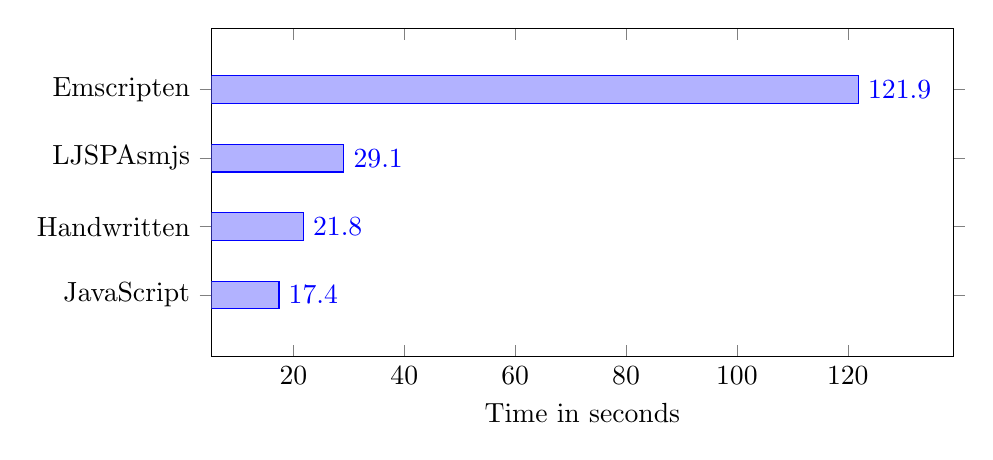
\begin{tikzpicture}
  \begin{axis}[
    xbar, xmax=139,
    width=11cm, height=5.75cm, enlarge y limits=0.3,
    xlabel={Time in seconds},
    symbolic y coords={JavaScript,Handwritten,LJSPAsmjs,Emscripten},
    ytick=data,
    nodes near coords, nodes near coords align={horizontal},
    ]
    
    \addplot coordinates {(17.4,JavaScript) (21.8,Handwritten) (29.1,LJSPAsmjs) (121.9,Emscripten)};
  \end{axis}
\end{tikzpicture}


  
  \caption{Rendering times of the four rendering methods}
  \label{benchmarksgraph}
\end{figure}

The first remarkable discovery we made using the ray tracer as benchmarking tool is that using the handwritten asm.js version turned out to be $24.9\%$ slower than using plain JavaScript to render the scene. This was a surprising result and went very much against our expectations.

The asm.js code generated by our compiler is $33.5\%$ slower than the handwritten asm.js version. This is a result that we are very happy with, especially considering that the first working version of the LJSP compiler produced code that made the rendering take more than 60 seconds. With more and better optimisation stages, we are confident that the generated code could get even closer to the handwritten, optimal version. It is not likely, however, to reach the performance of plain JavaScript, as not even the optimal version could get close to that.

The code generated by Emscripten from the C code the LJSP compiler generates is much slower than the other three versions, taking over two minutes on average to render the scene. It is $319.4\%$ slower than the asm.js code generated by the LJSP compiler directly and $459.7\%$ slower than the handwritten version. We strongly suspect that this is because Emscripten comes with a runtime that comes with a big overhead compared to the simple asm.js code the other two asm.js files are written in. This is reflected in the size of the files: The file that Emscripten generates is 4840 lines in total, whereas the handwritten version fits into 74 lines.

We suspect that the overhead generated by repeatedly calling asm.js code from JavaScript is one of the reasons the version written in plain JavaScript is faster than even the optimal asm.js version. Additionally, current JavaScript engines already produce very efficient code for functions like \texttt{raySphereIntersectionPoint} that consist of simple mathematical operations.

Based on these disoveries and theories, we assume that the true strength of asm.js lies in being a compilation target for complex apps, such as the gaming engine compiled in the example that Mozilla gives on their webpage. Breaking down complex code, such as object oriented C++, into simple asm.js during compilation and executing the resulting machine code is much faster as translating the C++ code to high level JavaScript as the benchmarks by Mozilla and others show \cite{asmjsbenchmarks}.

It is still surprising to us, however, that asm.js performs so badly in our use case. The fact that asm.js code is limited to arithmetic operations and read/write access to an array is one of the sources for criticism \cite{adblock, whybothers} of it. We believe that this is also why, despite the initial hype, it hasn't yet achieved any serious level of adoption. Outside of a relatively small niche of applications such as gaming engines and possibly cryptography, asm.js is not expressive enough. The developers of asm.js seem to be aware of this and David Herman, one of its developers, has addressed this problem with a list of planned additions to the specification at \cite{asmjsadditions} such as garbage collection and binary data handling in early 2013.

\section{Evaluating the Compiler}

% TODO LIB somewhere else: During the development of the LJSP compiler, edge cases like this arose frequently and had to be solved with small hacks.
% also: types?

While originally only conceived to compile LJSP to asm.js, the compiler was later extended to compile LJSP to C and LLVM IR as well. This decision was made after seeing the first benchmarks and was motivated by a desire to get a fuller picture of asm.js running times. Because Emscripten includes heavy optimisation, we thought it might produce code that runs faster than the code generated by the LJSP, which later turned out not to be the case. The reason both C and LLVM IR are included as back ends is a remnant of the development of the compiler. When developing the LLVM IR back end, we chose to first output C code, which is easier to generate because it is closer to the Intermediate Representation. We then compiled the C code this back end generated to LLVM IR using clang\footnote{clang is the C compiler of the LLVM project.}. Using the output of clang as a reference, we added a second back end for LLVM IR to the LJSP compiler that imitates the output that clang generates. Because the LJSP compiler performs no optimisations when compiling from C to LLVM IR, the code these two back ends generate is equivalent in the operations it performs with the generated LLVM IR being more low-level and explicit. When compiling to asm.js using Emscripten, we used the output generated by the C back end and the \texttt{emcc} binary that comes with the Emscripten distribution.

Projects that grow beyond their initial scope on often turn into an unorganised patchwork. We are generally happy with how the compiler turned out after all extensions. It was, however, necessary to rewrite and refactor significant parts of the program at various points during the project to accomodate for new requirements. An example of this is the Intermediate Representation and the related stages that were not part of the first version of the compiler. They only became necessary after C was implemented as an additional compilation target, to remove code duplication among asm.js and C conversion and combine the shared changes that both stages made to the AST into one parent stage.

Using Scala to implement the compiler turned out to generally have been a good choice. Scala's pattern matching expression is very well suited for writing a compiler and is used throughout the LJSP compiler. The possibility to mix functional and imperative programming styles was helpful and often resulted in expressive and elegant code. The downside of using Scala was the slow execution speed of the Scala compiler. This became a bigger and bigger problem as the project grew in size. Compiling the LJSP project in its current form takes almost 40 seconds on our machine, which made it no longer possible to make small incremental changes to the compiler and instead required us to batch together a number of changes before compiling. Additionally, on some occurences, the Scala compiler segfaulted for unknown reasons, which was fixed by rerunning it with the same arguments.

The biggest design mistake made during the development of the LJSP compiler was to make all parameters to C functions to be of type \texttt{void*} instead of deriving their types from the way they are used inside the function body. Doing so would have made the C code easier to generate, less complex and possibly substantially faster. It would have avoided the need for much of the complex pointer handling and some memory management. It also would not have been difficult to implement, because type derivation is already done for all local variables and could easily have been extended to include parameters as well. The reason we decided to make all parameters of the same type was because that is how the asm.js conversion stage, that had been implemented earlier, was designed. It worked well for asm.js, but it was not an optimal choice for C. Implementing type derivation for parameters, removing most of the calls to \texttt{jalloc} and compiling the code again with Emscripten would yield an interesting additional data point.

Another aspect of the compiler that could be improved is related to the fact that there is a substantial number of stages that only change expressions of a small number of types while leaving the remaining expressions unaltered: "Reduction of Primitive Operations" only touches prim ops, "Closure Conversion" only changes lambas and applications. To traverse the entire Abstract Syntax Tree, these stages need to handle every kind of expression, however, so that subexpressions can be examined. Closure converting the expression \texttt{(if $e_1$ $e_2$ $e_3$)}, for example, leaves the if untouched but gets called recursively for all three subexpressions $e_1$, $e_2$ and $e_3$. Separating the AST-traversing algorithm from the changes that every stage early on would have made the code much more concise. Sarkar, Waddell, and Dybvig describe \cite{nanopass} a mechanism they call "pass expander" that automatically generates code to handle expressions in each stage that don't change.

A further mistake that was made in the beginning and was later corrected was the unnecessary introduction of \texttt{lambda}s to the code during CPS-translation. This seemed to be a good idea from a theoretical perspective looking at the CPS-translation equations, but in practise, it turned out to be very slow. Specifically in the case of \texttt{if}-expressions, described in detail in the CPS-translation section of the Implementation Chapter, it turned out that the trade-off between speed and code duplication did not exist in reality. Introducing additional \texttt{lambda}s made the code not just slower, but eventually also longer, because calling them requires lengthy construction of closures.

Much of the initial difficulty in developing the compiler was in understanding the concept of Continuation-Passing Style and a lot of time was spent on finishing the three main front end stages: CPS-translation, closure conversion and hoisting. After that part of the project was completed, reading and understanding the asm.js specification turned out to be another challenge as the material on asm.js is limited and quite terse.

In conclusion, we are satisfied with the results that the project has achieved. Our initial requirements were met and the question we set out with was answered. The results the project generated could be developed further in ways that we will describe in the next chapter.

\chapter{Conclusions}
This chapter will recapitulate the report and summarise the scope and findings of the project. It will also give an overview of possible future work on the LJSP project.
\section{What we have done}

With this project, we set out to evaluate asm.js as a compilation target for a relatively simple language called LJSP. We wrote a compiler for LJSP that compiles to asm.js and also implemented a ray tracer in JavaScript to have a benchmark that would allow us to compare different versions of the code.

The initial result of asm.js code being much slower than plain JavaScript were surprising and going against our expectations. Although we were able to much improve the asm.js code generated by our compiler, this performance gap did not go away. 

To get another data point, we extended our compiler to also be able to generate C and LLVM IR code from LJSP so that we could then pass this output on to the Emscripten compiler. The results this generated were again surprising by being much slower than any other version of the ray tracer the project includes.

Rewriting the code in asm.js by hand revealed that even an optimal asm.js version was still slower than the version that used standard JavaScript only.

Our hypothesis is that asm.js is not suited for the kind of purpose we used it for: small functions that compute some relatively simple arithmetic operations, called repeadedly from standard JavaScript.

\section{Future Work}

The next step in evaluating asm.js would be to extend LJSP's grammar so that the entire ray tracer could be written in LJSP. This would cause more complex object oriented code to be compiled to asm.js and would also reduce the interaction between asm.js and non-asm.js JavaScript. The first step to reach this goal would be to implement lists.

Another addition to the project that would have to be made soon, should development on it continue, is an interpreter for the Intermediate Representation. This would then make it possible to include the intermediate stages in the stages covered by the testing framework.

Finally, more intermediate stages could be added that optimise the generated code more heavily such as tail call elimination. The intermediate representation that is already part of the compiler offers a suitable framework for adding such stages. This would depend on the addition proposed in the previous paragraph, as these new stages would have to be tested to be reliable. Especially optimisation stages are prone to contain errors and keeping these new stages as small as possible, as described in \cite{nanopass2} would make testing and debugging them easier.

\chapter{User Guide}

This chapter will describe the commands necessary to achieve the result presented in the Evaluation and other earlier chapters.
\section{Compiler}
The first step before the compiler can be used is to compile the compiler. This is done by calling \texttt{scalac -deprecation ./*.scala} from the root directory of the repository. We have included an executable version that was compiled with Scala version 2.9.1-1. Compiling the compiler will take some time (around 37 seconds on a 1.6 GHz MacBook Air).

After it has been compiled, the LJSP compiler can be called by entering \texttt{scala -cp ljsp/ ljsp.Ljsp} on the command line. Executing that command, without any switches, prints the usage of the compiler that shows all switches that are available.

These available command line arguments comprise:
\begin{itemize}
\item Either \texttt{-i} followed by a file name that contains LJSP code or code in a string, e.g. \texttt{scala -cp ljsp/ ljsp.Ljsp "(define (add x y) (+ x y))(add 1 2)"} but not both.
\item One compilation target. The full list of possible targets can be views by calling the compiler without arguments and corresponds to the list of stages in the compiler. If no target is given, all targets are printed to the command line.
\item Optionally, \texttt{-o} followed by an output file name that the result of the compilation should be written to.
\end{itemize}

\section{Ray Tracer}

The ray tracer can be used by opening the \texttt{ray_tracer/ray_tracer.html} file in a recent version of Firefox\footnote{During the development of the ray tracer, Firefox 27 was used.}. Clicking on one of the four buttons will render a 3D scene with the rendering method selected. Please note that the renderer will not show anything until the renderer has finished. 

The HTML file depends on a number of JavaScript files, all of which are included in the repository. Two of these files can, however, be generated by compiling the \texttt{ray_tracer/ljsp_code.scm} file.

The first of these files is the JavaScript file containing the asm.js code for rendering the scene using asm.js code generated by the LJSP compiler (the rendering method activated by the third of the four buttons). This file is called \texttt{ray_tracer/gen_code.js} and can be generated by executing the following command from the root of the repository: \texttt{scala -cp ljsp/ ljsp.Ljsp --asmjs -i ray_tracer/ljsp_code.scm -o ray_tracer/gen_code.js}. Please note that the LJSP compiler must have been successfully compiled, before it can be used. See the first section of this chapter for details on how to do this.

The second file contains the asm.js code generated by Emscripten (the forth of the four buttons renders the scene using this implementation). To generate this file, an Emscripten compatible C version of the \texttt{raySphereIntersectionPoint} has to be generated using the LJSP compiler by calling \texttt{scala -cp ljsp/ ljsp.Ljsp --emC -i ray_tracer/ljsp_code.scm -o rtc.c} from the root of the repository. This generated a file called \texttt{rtc.c}, also included with the repository. To compile this file and save the result in \texttt{ray_tracer/emcc_output.js}, which is where the ray tracer expects the Emscripten code, call Emscripten with this command: \texttt{emcc -O2 -s EXPORTED_FUNCTIONS="['_raySphereIntersectionPoint_copy_call_by_value', '_vectorsDotProduct_copy_call_by_value']" -s NO_EXIT_RUNTIME=1 rtc.c -o ray_tracer/emcc_output.js}. For this command to work, Emscripten must be installed and \texttt{emcc} in the \texttt{PATH}. For instructions on how to install Emscripten, please see the Emscripten tutorial\footnote{https://github.com/kripken/emscripten/wiki/Tutorial}.

\section{Testing}
Running tests can be achieved by executing \texttt{python run_tests.py} on the command line. This requires Python 2 to be installed. The testing framework further depends on Racket and LLVM to be installed on the machine. \texttt{run_tests.py} contains two constants \texttt{RACKET_PATH} and \texttt{LLI_PATH} that point to the executables of racket\footnote{Racket can be downloaded at http://download.racket-lang.org/} and lli\footnote{lli is the LLVM IR interpreter that comes with the LLVM project which can be downloaded at http://llvm.org/releases/download.html}. These constants need to be adjusted to contain the correct paths.


\newpage
\chapter{Bibliography}
% TODO END make this beautiful, maybe two column format
\begin{thebibliography}{1}
    \bibitem{githubarchive} {\em GitHub Archive} http://www.githubarchive.org/ accessed on 28.3.2014.
    \bibitem{topgithub} {\em Top Github Languages for 2013 (so far)} http://adambard.com/blog/top-github-languages-for-2013-so-far/ accessed on 28.3.2014
    \bibitem{jsgoodparts} Douglas Crockford (2008) {\em JavaScript: The Good Parts, Unearthing the Excellence in JavaScript}, pp. 101
    \bibitem{sysftal} Morrisett, Greg and Walker, David and Crary, Karl and Glew, Neal (1999). {\em From System F to Typed Assembly Language}, ACM Trans. Program. Lang. Syst.
    \bibitem{brendeich} Foreword by Brendan Eich to {\em Node: Up and Running}. Available at http://chimera.labs.oreilly.com/books/1234000001808/pr02.html accessed on 28.3.2014.
    \bibitem{appel} Andrew Appel (1992). {\em Compiling with Continuations} Cambridge University Press
    \bibitem{asmjsbenchmark} Alon Zakai, {\em Big Web App? Compile it!} http://kripken.github.com/mloc_emscripten_talk/\#/28 mloc.js JavaScript Conference 2013, accessed on 30.3.2014
    \bibitem{unreal} 27.3.2013, {\em Mozilla is Unlocking the Power of the Web as a Platform for Gaming} https://blog.mozilla.org/blog/2013/03/27/mozilla-is-unlocking-the-power-of-the-web-as-a-platform-for-gaming/ accessed on 9.4.2014
    \bibitem{physrendering} Matt Pharr, Greg Humphreys (2010) {\em Physically Based Rendering, 2nd edition} pp. 116
    \bibitem{comparticle} Charles Severance {\em JavaScript: Designing a Language in 10 Days} Computer, vol. 45, no. 2, pp. 7-8, Feb., 2012 
    \bibitem{asmjsspec} {\em asm.js specification - Working Draft} http://asmjs.org/spec/latest/ accessed on 9.4.2014
    \bibitem{asmjspdf} Dave Herman, Luke Wagner, and Alon Zakai {\em asm.js: a High Performance Subset of JavaScript} https://github.com/dherman/asm.js/blob/master/tex/def.pdf accessed on 9.4.2014
    \bibitem{emscriptenpapar} Alon Zakai, {\em Emscripten: An LLVM-to-JavaScript Compiler} 'OOPSLA Companion' , ACM, , pp. 301-312
    \bibitem{onlisp} Paul Graham, {\em On Lisp}, Prentice Hall, 1993, p. 260
    \bibitem{findingbugsinccomp} John Regehr et al., {\em Finding and Understanding Bugs in C Compilers}, ACM SIGPLAN Conference on Programming Language Design and Implementation (PLDI), San Jose, CA, Jun. 2011
    \bibitem{compcert} Xavier Leroy {\em Formal verification of a realistic compiler}, Commun. ACM, 2009
    \bibitem{nanopass} Sarkar, D.; Waddell, O. \& Dybvig, R. K. (2004), {\em A nanopass infrastructure for compiler education}, in Chris Okasaki \& Kathleen Fisher, ed., 'ICFP', ACM, pp. 201-212
    \bibitem{nanopass2} Keep, Andrew W. and Dybvig, R. Kent (2013), {\em A Nanopass Framework for Commercial Compiler Development}, in 'ICFP', ACM, pp. 343-350
    \bibitem{hnthread} Hacker News asm.js release thread, https://news.ycombinator.com/item?id=5227274 accessed on 13.4.2014
    \bibitem{asmjsbenchmarks} Asm.js benchmarks and comparisons, http://arewefastyet.com/\#machine=11\&view=breakdown\&suite=asmjs-apps accessed on 13.4.2014
    \bibitem{adblock} Wladimir Palant, {\em Thoughts on using asm.js for performance bottlenecks in browser extensions} https://adblockplus.org/blog/thoghts-on-using-asmjs-for-performance-bottlenecks-in-browser-extensions accessed on 13.4.2014
    \bibitem{asmjsadditions} David Herman on future plans for asm.js https://news.ycombinator.com/item?id=5228042 accessed on 13.4.2014
    \bibitem{whybothers} Vyacheslav Egorov, March 2013 {\em Why asm.js bothers me} http://mrale.ph/blog/2013/03/28/why-asmjs-bothers-me.html accessed on 13.4.2014
\end{thebibliography}

\end{document}
